\documentclass[aspectratio=169,10pt]{beamer}

% Import all packages
%%%%%%%%%%%%%%%%%%%%%%%%%%%%%%%
%     import des packages     %
%%%%%%%%%%%%%%%%%%%%%%%%%%%%%%%
\usepackage[export]{adjustbox}
\usepackage{amsmath,amsfonts,amssymb}
\usepackage{anyfontsize}
\usepackage{array}
\usepackage[french]{babel}
\usepackage{bbm}
\usepackage{colortbl}
\usepackage{comment}
\usepackage{cclicenses}
\usepackage{eqnarray}
\usepackage{eso-pic}
\usepackage{enumerate} % Pour personnaliser les énumération
\usepackage{fancybox}
\usepackage{fancyhdr}
\usepackage{float}
\usepackage[T1]{fontenc} 
\usepackage{forest}
\usepackage{gensymb}
\usepackage{geometry}
\usepackage{glossaries}
\usepackage{graphicx}
\usepackage{hyperref}
\usepackage{ifthen}
\usepackage{import}
\usepackage{indentfirst}
\usepackage[utf8]{inputenc}
\usepackage{lastpage}
\usepackage{libertine}
\usepackage{lipsum}
\usepackage{listings}
\usepackage{lmodern}
\usepackage{mathtools}
\usepackage{mdframed}
\usepackage{multicol}
\usepackage{pdfpages}
\usepackage{pifont}
\usepackage{stmaryrd}
\usepackage{subcaption}
\usepackage{subfiles}
\usepackage{tabularx}
% \usepackage{tcolorbox}
\usepackage[most]{tcolorbox}
\usepackage[absolute,overlay]{textpos} % To position the image
\usepackage{textcomp}
\usepackage{ulem}
\usepackage{wrapfig}
\usepackage{xcolor}


\newcommand{\titre}{Conception et optimisation d'algorithmes de coordination multi-robots}
\newcommand{\titrefooter}{Soutenance - Projet de fin d'études}
\newcommand{\soustitre}{Exploration autonome de réseaux de galeries}
\newcommand{\auteur}{Fabien MATHÉ}
\newcommand{\referent}{M. Mehmet ERSOY}
\newcommand{\institut}{SeaTech - MOCA 3A}
\newcommand{\presentationdate}{27 février 2025}


% Thème clair et épuré
\usetheme{Berlin} % Thème Berlin
\usecolortheme{seahorse}
\setbeamertemplate{navigation symbols}{} % Suppression des symboles de navigation

% Personnalisation du thème

% Couleurs personnalisées
\definecolor{mainblue}{RGB}{0, 102, 204} % Bleu principal
\definecolor{lightgray}{RGB}{240, 240, 240} % Gris clair
\definecolor{darkgray}{RGB}{100, 100, 100} % Gris plus foncé pour les points non actifs
\definecolor{lightblue}{RGB}{173, 216, 230} % Bleu clair
\definecolor{darkblue}{RGB}{0, 51, 102} % Bleu foncé

% Configuration des couleurs
% \setbeamercolor{normal text}{bg=white, fg=black}
% \setbeamercolor{structure}{fg=mainblue}
% \setbeamercolor{frametitle}{bg=lightgray, fg=mainblue}
% \setbeamercolor{title}{fg=mainblue}
% \setbeamercolor{itemize item}{fg=mainblue}

% Personnalisation des couleurs du thème
\setbeamercolor{normal text}{bg=white, fg=black} % Texte principal en gris foncé sur fond blanc
\setbeamercolor{structure}{fg=mainblue} % Couleur principale des titres (sections, sous-sections)
\setbeamercolor{frametitle}{bg=lightgray, fg=mainblue} % Titre des frames avec fond bleu clair et texte bleu
\setbeamercolor{title}{fg=mainblue} % Couleur du titre principal
\setbeamercolor{itemize item}{fg=mainblue} % Couleur des puces (items)
\setbeamercolor{enumerate item}{fg=mainblue} % Couleur des items des listes numérotées
\setbeamercolor{section in toc}{fg=mainblue} % Sections dans la table des matières
\setbeamercolor{subsection in toc}{fg=darkblue} % Sous-sections dans la table des matières

% Personnalisation des blocs de couleur
\setbeamercolor{block title}{bg=mainblue, fg=white} % Titre des blocs avec fond bleu et texte blanc
\setbeamercolor{block body}{bg=lightblue, fg=black} % Corps des blocs avec fond bleu clair et texte noir
\setbeamercolor{alertblock title}{bg=darkblue, fg=white} % Titre des alertes avec fond bleu foncé et texte blanc
\setbeamercolor{alertblock body}{bg=lightblue, fg=black} % Corps des alertes avec fond bleu clair et texte noir
\setbeamercolor{exampleblock title}{bg=mainblue, fg=white} % Titre des exemples avec fond bleu et texte blanc
\setbeamercolor{exampleblock body}{bg=lightblue, fg=black} % Corps des exemples avec fond bleu clair et texte noir

% \setbeamercolor{palette primary}{use=structure,fg=white,bg=structure.fg}
% \setbeamercolor{palette secondary}{use=structure,fg=white,bg=structure.fg!75}
% \setbeamercolor{palette tertiary}{use=structure,fg=white,bg=mainblue}
% \setbeamercolor{palette quaternary}{fg=white,bg=mainblue}

% Modification des puces (bulles) dans les listes
\setbeamertemplate{itemize item}[circle] % Change les puces classiques en cercles
%\setbeamertemplate{itemize item}[square] % Change les puces en carrés
%\setbeamertemplate{itemize item}[triangle] % Change les puces en triangles
%\setbeamertemplate{itemize item}[rectangle] % Change les puces en rectangles

% Modification des numéros dans les listes numérotées (enumerate)
\setbeamertemplate{enumerate item}[circle] % Change les numéros en cercles
%\setbeamertemplate{enumerate item}[square] % Change les numéros en carrés
%\setbeamertemplate{enumerate item}[triangle] % Change les numéros en triangles
%\setbeamertemplate{enumerate item}[rectangle] % Change les numéros en rectangles


% Bas de page personnalisé (nom, établissement, date, numéro de page)
\newcommand{\customfootline}{
	\setbeamertemplate{footline}{
		\begin{beamercolorbox}[ht=2ex, dp=1ex]{}
			\colorbox{lightgray}{
				\parbox{\textwidth}{
					\begin{minipage}{0.19\linewidth}
						\centering
						\auteur
					\end{minipage}
					\hfill
					\begin{minipage}{0.19\linewidth}
						\centering
						\institut
					\end{minipage}
					\hfill
					\begin{minipage}{0.19\linewidth}
						\centering
						\titrefooter
					\end{minipage}
					\hfill
					\begin{minipage}{0.19\linewidth}
						\centering
						\presentationdate
					\end{minipage}
					\hfill
					\begin{minipage}{0.19\linewidth}
						\centering
						\insertframenumber/\inserttotalframenumber
					\end{minipage}
					\vspace{0.5em}
				}
			}
		\end{beamercolorbox}
	}
}


% Titre de la présentation
\title[Titre court]{\titre}
\subtitle{\soustitre}
\author{\auteur}
\institute{\institut \newline \titrefooter}
\date{\presentationdate}

\usefonttheme[onlymath]{serif}

\begin{document}

% Page de titre (Timeline non affichée ici)

\setbeamertemplate{headline}{}
\setbeamertemplate{footline}{}

\begin{frame}
    \titlepage
\end{frame}

\setbeamertemplate{headline}[miniframes theme]
\customfootline

% Section 1 : Introduction
\section{Introduction}

\begin{frame}{\textbf{Introduction}}
	\begin{minipage}{0.6\linewidth}
		\begin{itemize}
			\item Fascination pour l'inconnu
			\vspace{0.2cm}
			\item Meilleure compréhension de notre planète
			\vspace{0.2cm}
			\item Défis inhérents de l'exploration souterraine
			\begin{itemize}
				\item Accessibilité
				\vspace{0.2cm}
				\item Communication
				\vspace{0.2cm}
				\item Navigation
			\end{itemize}
			\vspace{0.2cm}
			\item Intérêt scientifique
			\begin{itemize}
				\item Découverte de nouvelles formes de vie
				\vspace{0.2cm}
				\item Structures géologiques préservées
			\end{itemize}
		\end{itemize}
	\end{minipage}
	\hfill
	\begin{minipage}{0.35\linewidth}
		\begin{figure}
			\centering
			\includegraphics[width=0.8\textwidth]{IMAGES/Grotte_de_la_flûte_de_pan.jpeg}
			\caption{Grotte de la flûte de pan (Guilin, Chine). Paul Munhoven \href{https://commons.wikimedia.org/w/index.php?curid=27712205}{\copyright}}
			\label{fig:china_cave}
		\end{figure}
	\end{minipage}

\end{frame}

\begin{frame}{\textbf{Introduction}}

	\begin{minipage}{0.6\linewidth}
		\begin{figure}
			\centering
			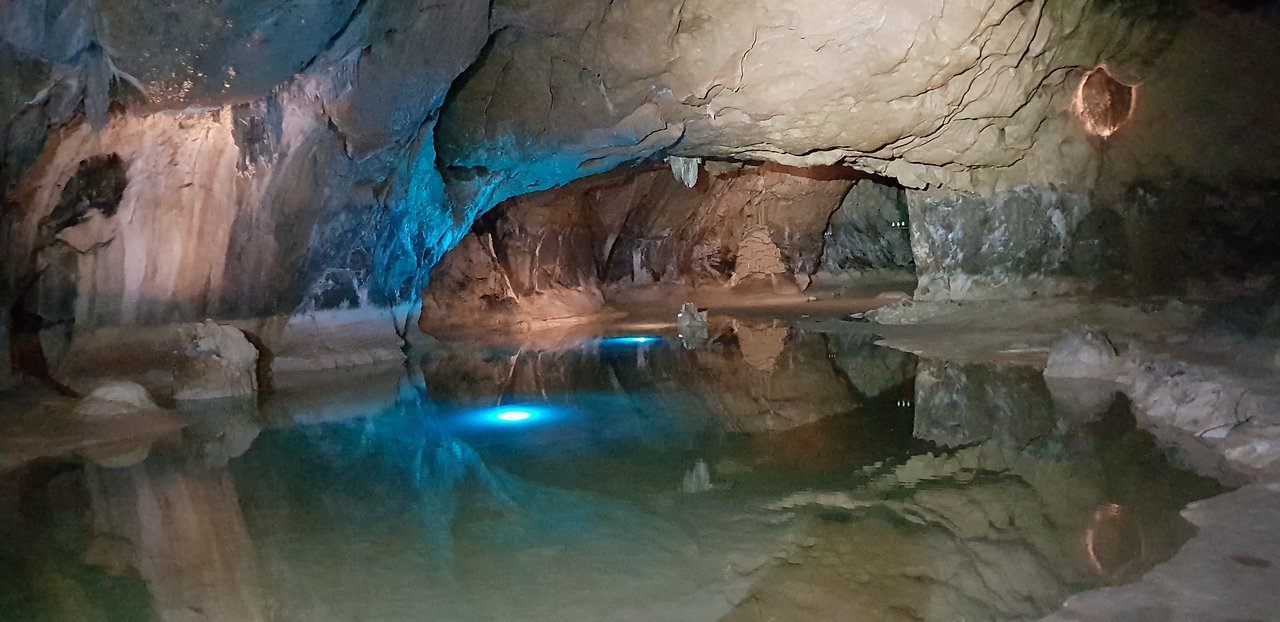
\includegraphics[width=0.8\textwidth]{IMAGES/le-lac-des-grottes-lombrives.jpg}
			\caption{Lac de la Grotte de Lombrives - Ariège}
			\label{fig:ariege_cave}
		\end{figure}
	\end{minipage}
	\hfill
	\begin{minipage}{0.35\linewidth}
		\begin{figure}
			\centering
			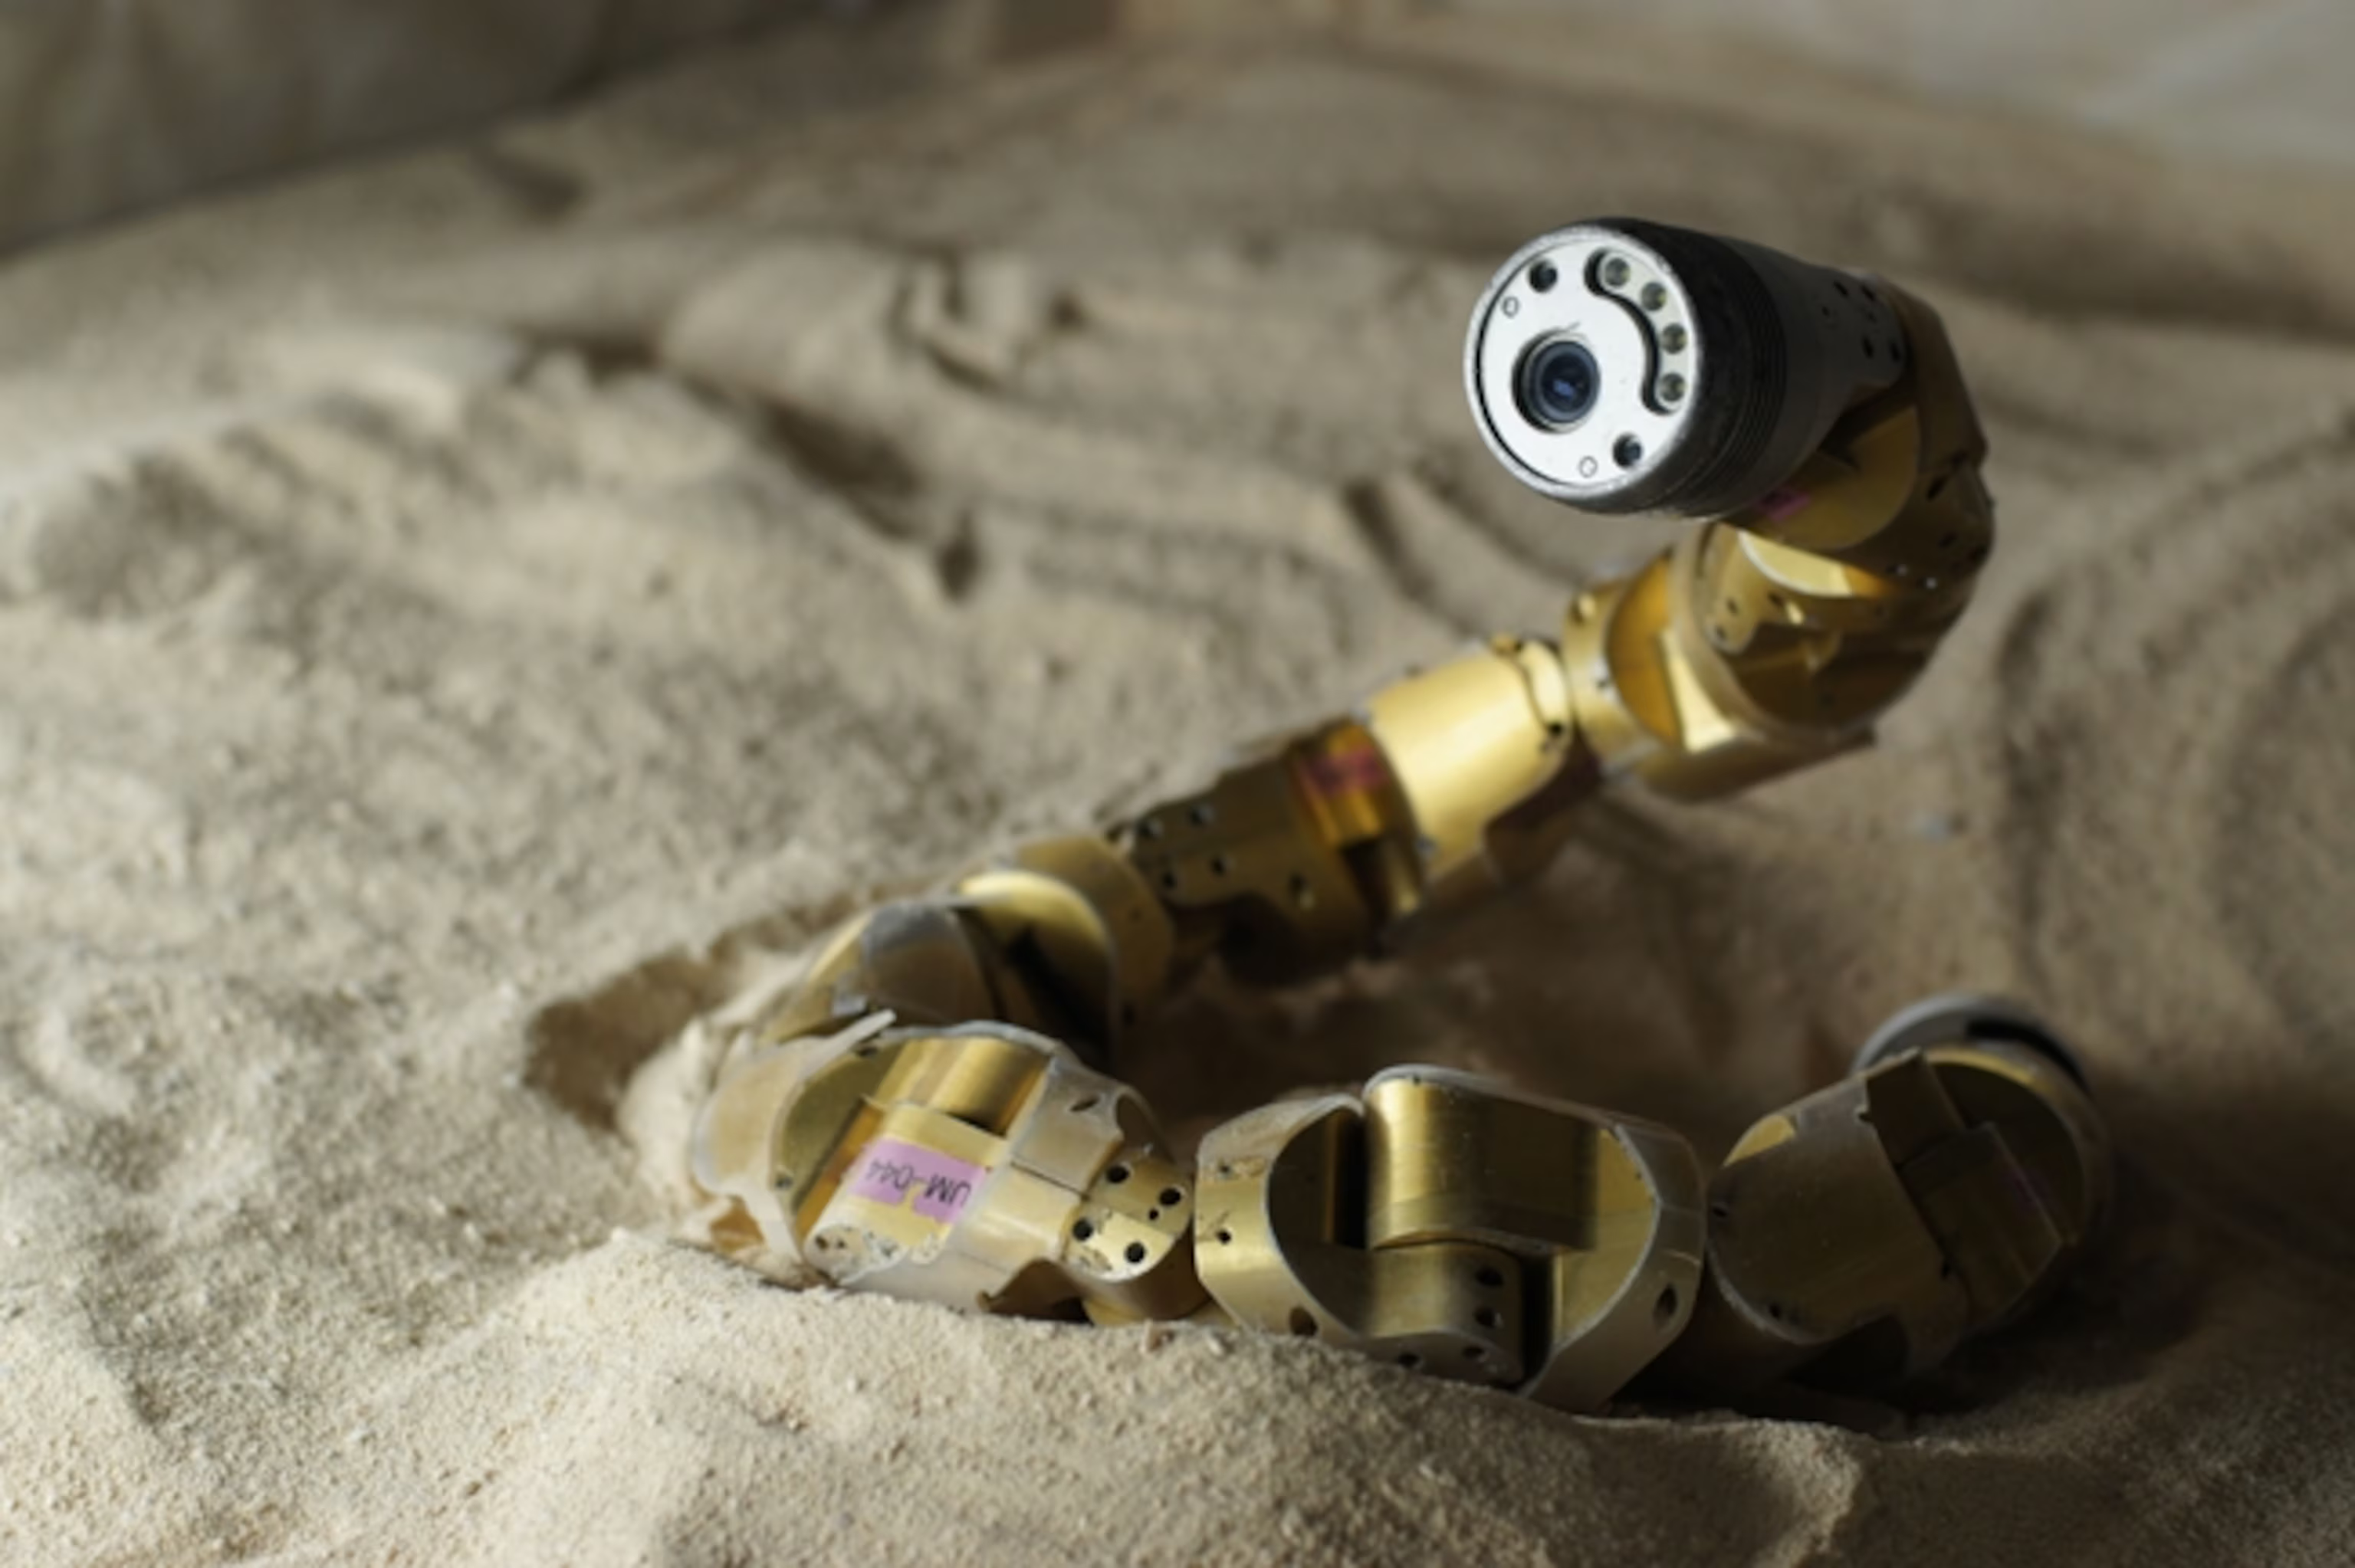
\includegraphics[width=0.9\textwidth]{IMAGES/Elizabeth.png}
			\caption{Elizabeth, le robot serpent. Nico Zevalios and Chaohui Gong}
			\label{fig:robot_exploration}
		\end{figure}
	\end{minipage}
    
	\textbf{Objectifs :}

	\vspace{0.8em}
	\begin{itemize}
		\item Développer des algorithmes de navigation pour des robots autonomes en milieu souterrain.
		\vspace{0.2cm}
		\item Assurer une communication autonome entre des robots sans contrôle externe.
	\end{itemize}
\end{frame}

% Table des matières
\begin{frame}{\textbf{Sommaire}}
    \tableofcontents
\end{frame}




%%%%%%%%%%%%%%%%%%%%%%%%%%%%%%%%%%%%%%%%%%%%%%%%%%%%%%%%%%%%%%%%%%%%%%%%%%%%%%%%
% Section 2
%%%%%%%%%%%%%%%%%%%%%%%%%%%%%%%%%%%%%%%%%%%%%%%%%%%%%%%%%%%%%%%%%%%%%%%%%%%%%%%%
\section{Planification de trajectoire}

\begin{frame}{\textbf{Tentative d'optimisation théorique}}
	\textbf{Objectif}
	\vspace{0.5em}
	
	Trouver le plus court chemin permettant d'explorer une carte inconnue
	
	\vspace{0.5em}
	\begin{itemize}
		\item Contrainte :
		\begin{itemize}
			\item Évitement des obstacles
		\end{itemize}
		\vspace{0.2cm}
		\item Simplifications :
		\begin{itemize}
			\item Aucune contrainte liée au robot
			\vspace{0.2cm}
			\item Espace 2D
		\end{itemize}
	\end{itemize}
	
\end{frame}

\begin{frame}[t]{\textbf{Définition de l'espace étoilé}}
	\begin{minipage}[t]{0.6\linewidth}
		On définit :
		\begin{equation*}
			\displaystyle
			FV(t) = \left\{ \, (1 - l) \, \mathbf{X}(t) + l\, \mathbf{M}(t, \alpha) \,|\, l \in [0, 1], \alpha \in [0, 2 \pi[ \, \right\}
		\end{equation*}
			
		\begin{equation*}
			\mathbf{M}(t, \alpha) = \mathbf{X}(t) + R(t, \alpha) 
			\begin{pmatrix}
				\cos \alpha & 0\\
				0 & \sin \alpha\\
			\end{pmatrix} 
			\mathbf{X}(t)
		\end{equation*}
	
		Avec $R(t, \alpha)$ la distance minimale entre le robot et le plus proche point d'intersection à un mur, borné par $R_{\max}$.
	\end{minipage}
	\hfill
	\begin{minipage}[t]{0.38\linewidth}
		\begin{figure}
			\centering
			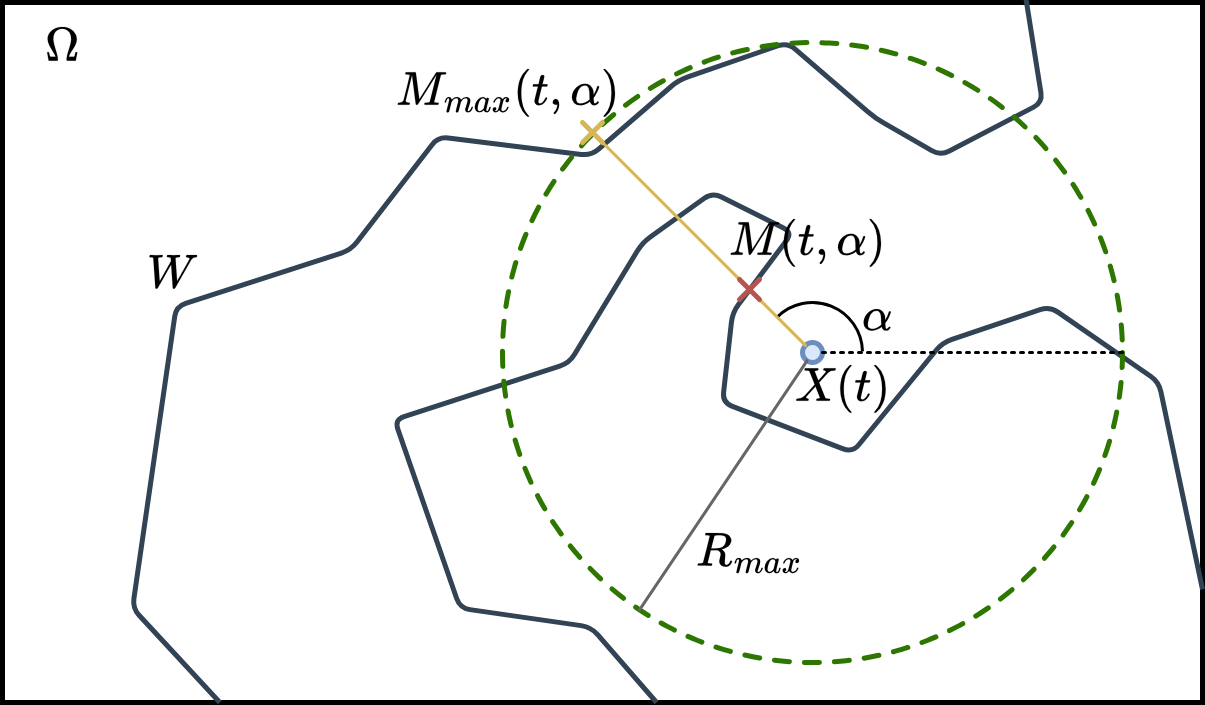
\includegraphics[width=\textwidth]{IMAGES/math_nota.png}
			\caption{Schéma des notations}
			\label{fig:math_notation}
		\end{figure}
	\end{minipage}
	
	\begin{itemize}
		\item $\displaystyle KM = \bigcup_{t=0}^{T} FV(t)$ : La partie de la carte connue par le robot
		\item $EM$ : La partie de la carte explorable par le robot
	\end{itemize}

\end{frame}

\begin{frame}{\textbf{Définition de la fonctionnelle et problèmes rencontrés}}
	\textbf{Fonctionnelle :}

	\begin{equation*}
		\displaystyle
		J(\mathbf{X}(0), T) = \int_{0}^{T} \| \mathbf{\dot{X}}(t) \| dt
	\end{equation*}

	avec pour contrainte $\mathbf{X}(0) = \mathbf{X}_{Robot}$, $\mathbf{X}(T) = \mathbf{X}_{WP}$, $KM(T) = EM$ et $\mathbf{\dot{X}}$ bornée.
	
	\begin{itemize}
		\item Comment garantir $\mathbf{X}(T)=\mathbf{X}_{WP}$ en contraignant $\dot{X}(t)$ ?
		\item Comment choisir le temps T ?
		\begin{itemize}
			\item T doit être suffisamment grand pour atteindre la cible.
			\item Si le robot s'arrête en $X_{WP}$ à $t = t_1$, alors :
			$$
			\displaystyle
			\int_{t_1}^{T} \| \mathbf{\dot{X}}(t) \| dt = 0
			$$
		\end{itemize}
		\item Comment prendre en compte l'exploration de la carte ?
	\end{itemize}
\end{frame}

\begin{frame}{\textbf{Proposition d'une nouvelle méthode}}
	\begin{figure}[H]
		\centering
		\begin{subfigure}[b]{0.3\textwidth}
			\centering
			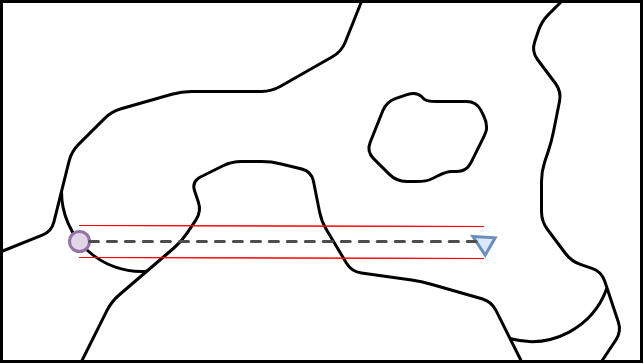
\includegraphics[width=\textwidth]{IMAGES/methode1.png}
			\caption{Tracer une ligne}
			\label{fig:draw_line}
		\end{subfigure}
		\hfill
		\begin{subfigure}[b]{0.3\textwidth}
			\centering
			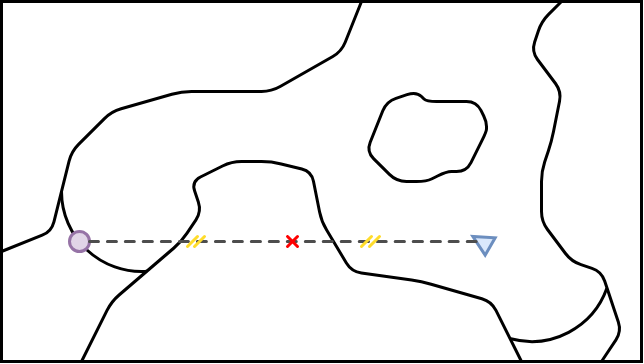
\includegraphics[width=\textwidth]{IMAGES/methode2.png}
			\caption{Vérifier si le chemin est libre}
			\label{fig:check_line}
		\end{subfigure}
		\hfill
		\begin{subfigure}[b]{0.3\textwidth}
			\centering
			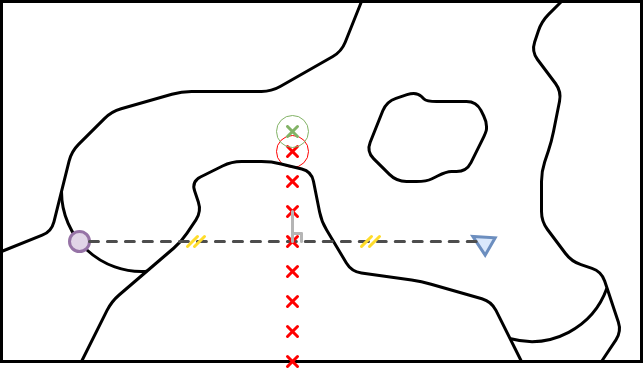
\includegraphics[width=\textwidth]{IMAGES/methode3.png}
			\caption{Tirer des points normaux}
			\label{fig:shoot_line}
		\end{subfigure}
		\vfill
		\begin{subfigure}[b]{0.3\textwidth}
			\centering
			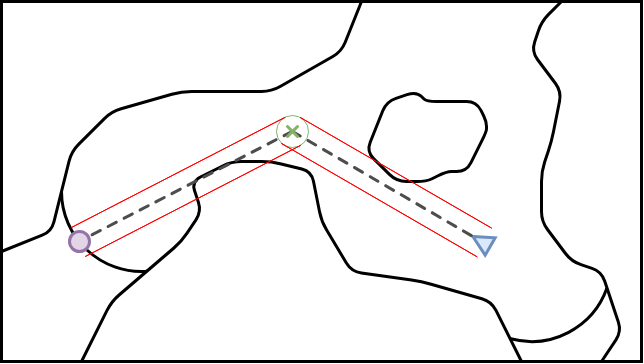
\includegraphics[width=\textwidth]{IMAGES/methode4.png}
			\caption{Valider le point}
			\label{fig:validate_point}
		\end{subfigure}
		\hfill
		\begin{subfigure}[b]{0.3\textwidth}
			\centering
			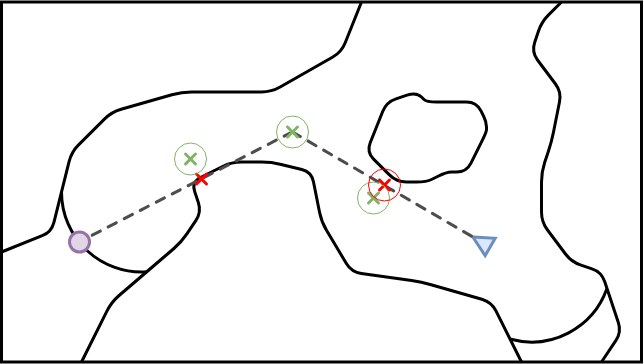
\includegraphics[width=\textwidth]{IMAGES/methode5.png}
			\caption{Répéter la méthode}
			\label{fig:repeat_method}
		\end{subfigure}
		\hfill
		\begin{subfigure}[b]{0.3\textwidth}
			\centering
			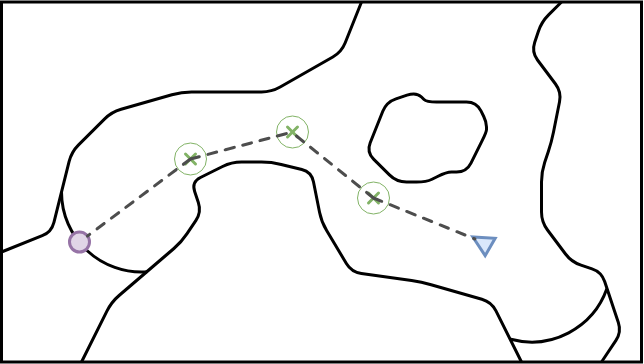
\includegraphics[width=\textwidth]{IMAGES/methode6.png}
			\caption{Connecter les points}
			\label{fig:idk}
		\end{subfigure}
		\caption{Visualisation de la méthode de recherche de chemin dynamique}
		\label{fig:method_visu}
	\end{figure}
\end{frame}

\begin{frame}{\textbf{Proposition d'une nouvelle méthode}}
    \begin{figure}[H]
		\centering
		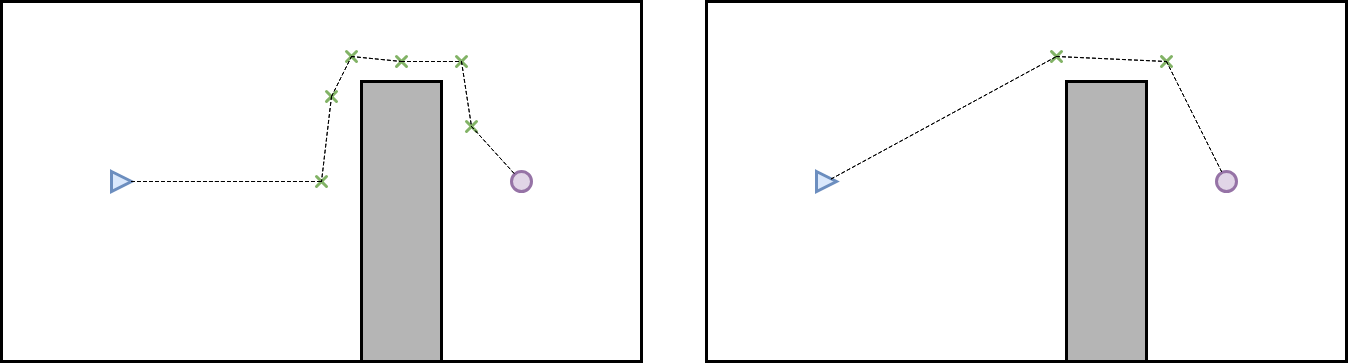
\includegraphics[width=0.7\textwidth]{IMAGES/shorten_path.png}
		\caption{Processus de simplification du chemin trouvé}
		\label{fig:path_simp}
	\end{figure}
\end{frame}

\begin{frame}{\textbf{Méthode de vérification}}
    Le chemin le plus court est modélisé par la propagation d'une onde à vitesse constante.\cite{tapia_2016}
	\begin{columns}[t]
		% Column 1
		\begin{column}{0.6\textwidth}
			\begin{itemize}
				\item Utilisation d'un automate cellulaire (CA)
				\vspace{0.2cm}
				\item La structure en réseau définit :
				\begin{itemize}
					\item Les cellules activées
					\vspace{0.1cm}
					\item Les obstacles
					\vspace{0.1cm}
					\item Les sources secondaires d'ondes
					\vspace{0.1cm}
					\item Les espaces vides
				\end{itemize}
				\item Un vecteur de distance suit la progression de l'onde.
				\vspace{0.2cm}
				\item Sources secondaires d'ondes ajoutées pour gérer les obstacles, inspirées du principe de Huygens.
			\end{itemize}
		\end{column}
		% Column 2    
		\begin{column}{0.4\textwidth}
			\begin{figure}
				\centering
				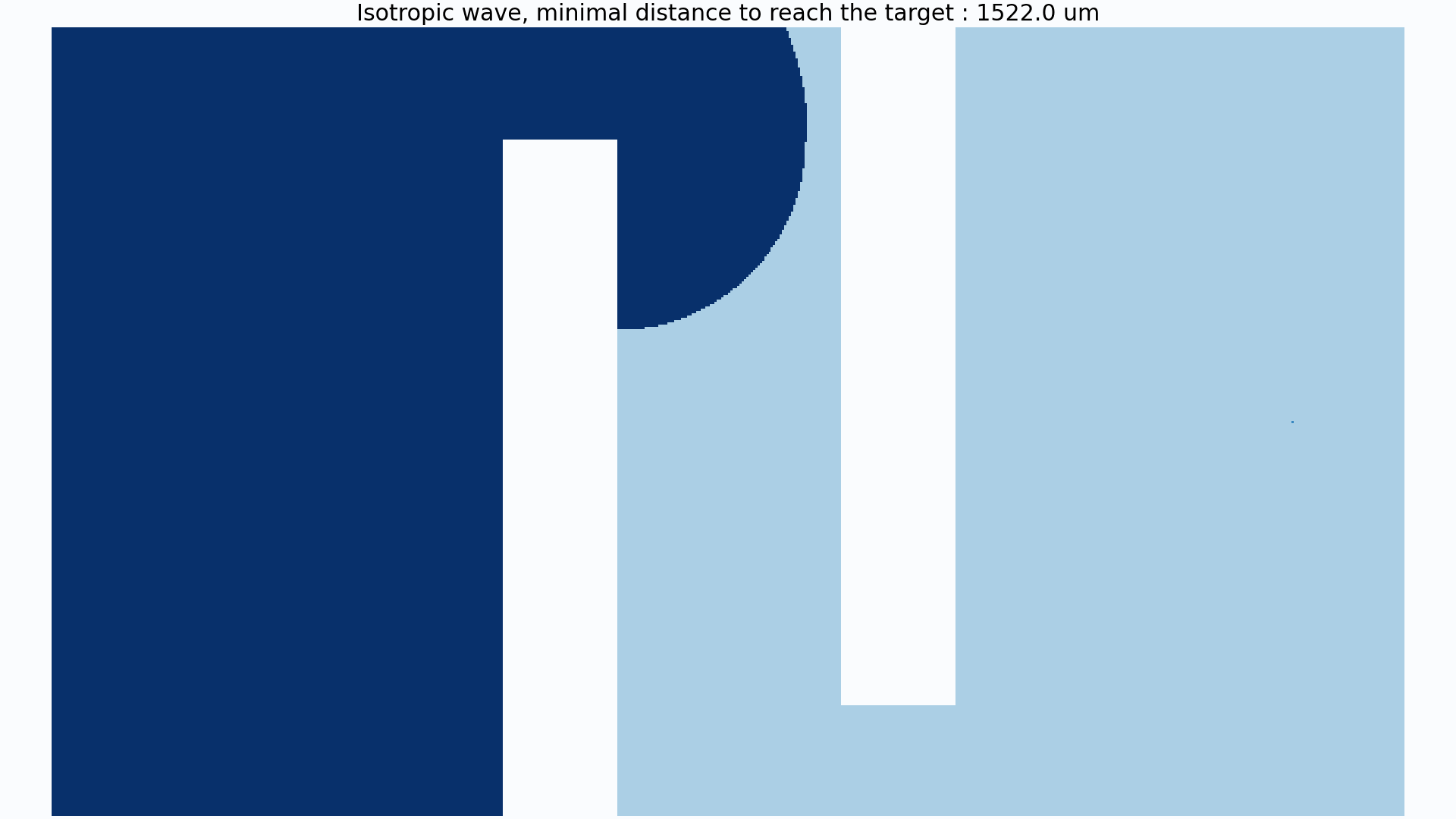
\includegraphics[width=\textwidth]{IMAGES/ca2.png}
				\label{fig:ca2}
				\caption{Propagation d'une onde à vitesse constante}
			\end{figure}
		\end{column}
	\end{columns}

\end{frame}

\begin{frame}{\textbf{Résultats et performance}}
    \begin{figure}[H]
		\centering
		\begin{subfigure}[b]{0.24\textwidth}
			\centering
			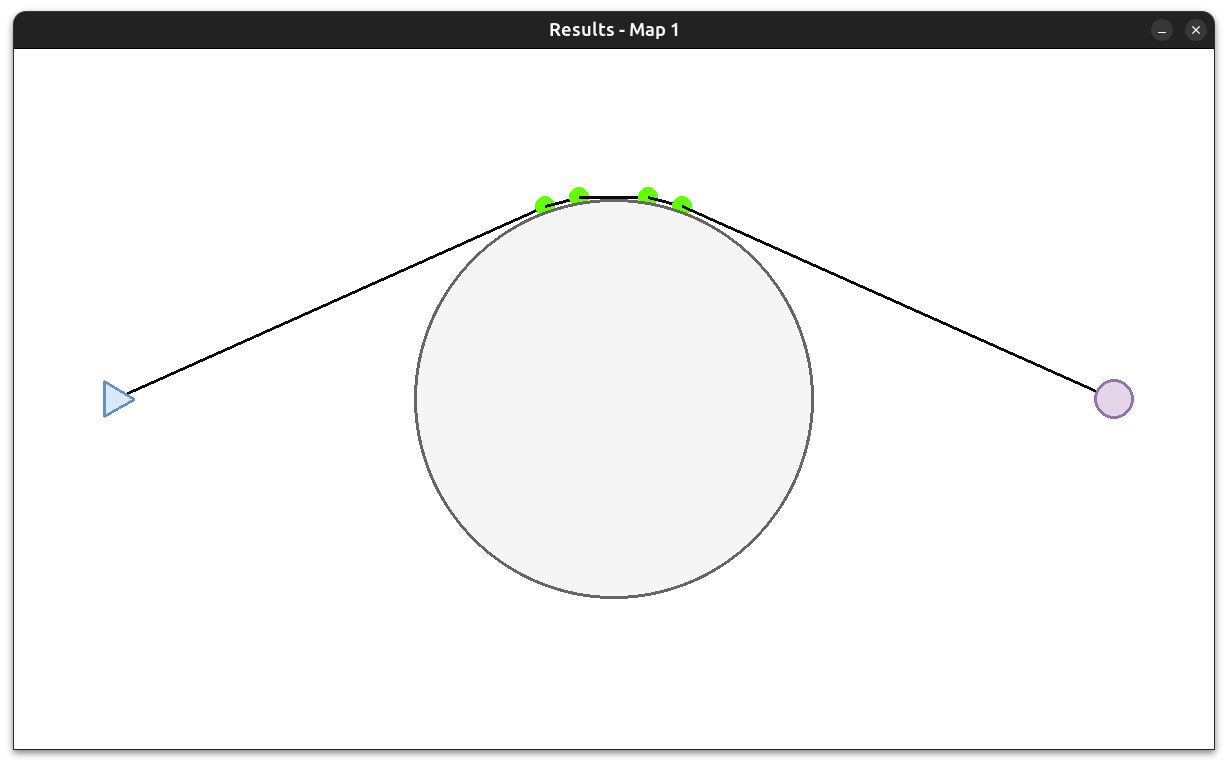
\includegraphics[width=\textwidth]{IMAGES/rmap1.png}
			\caption*{Résultats carte n°1}
			\label{fig:rmap1}
		\end{subfigure}
		\hfill
		\begin{subfigure}[b]{0.24\textwidth}
			\centering
			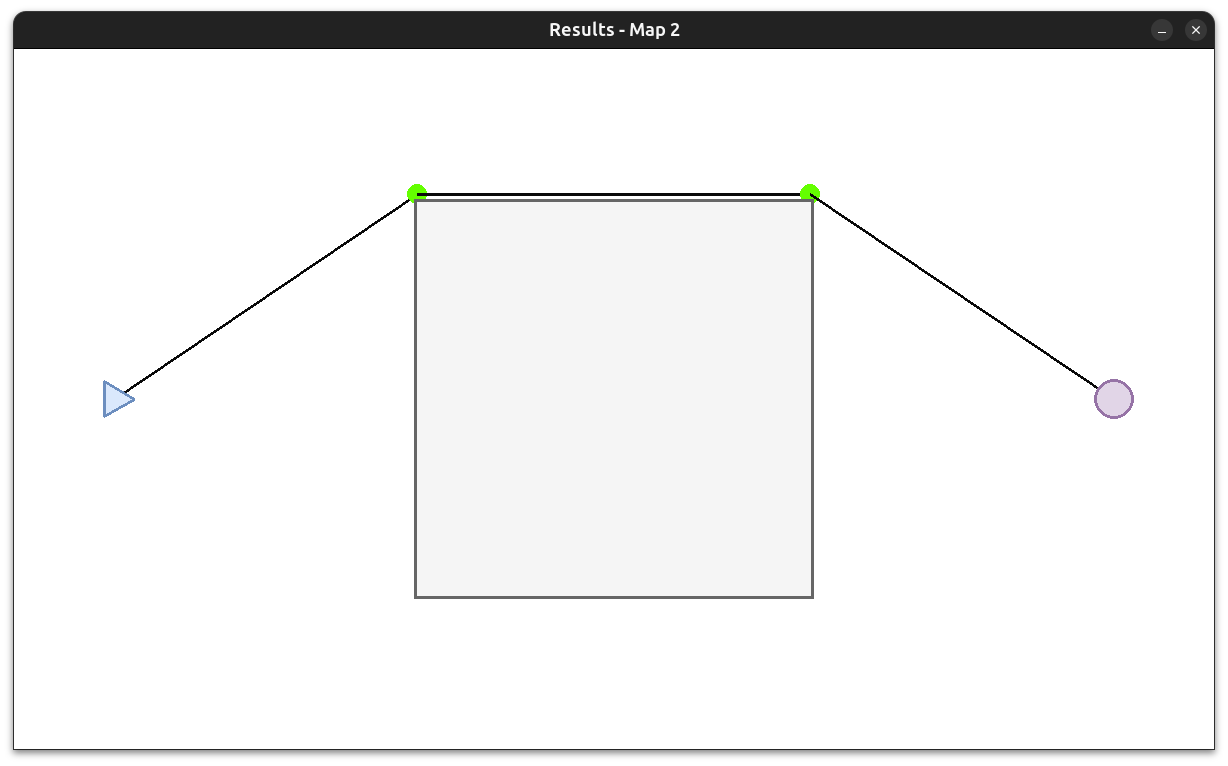
\includegraphics[width=\textwidth]{IMAGES/rmap2.png}
			\caption*{Résultat carte n°2}
			\label{fig:rmap2}
		\end{subfigure}
		\hfill
		\begin{subfigure}[b]{0.24\textwidth}
			\centering
			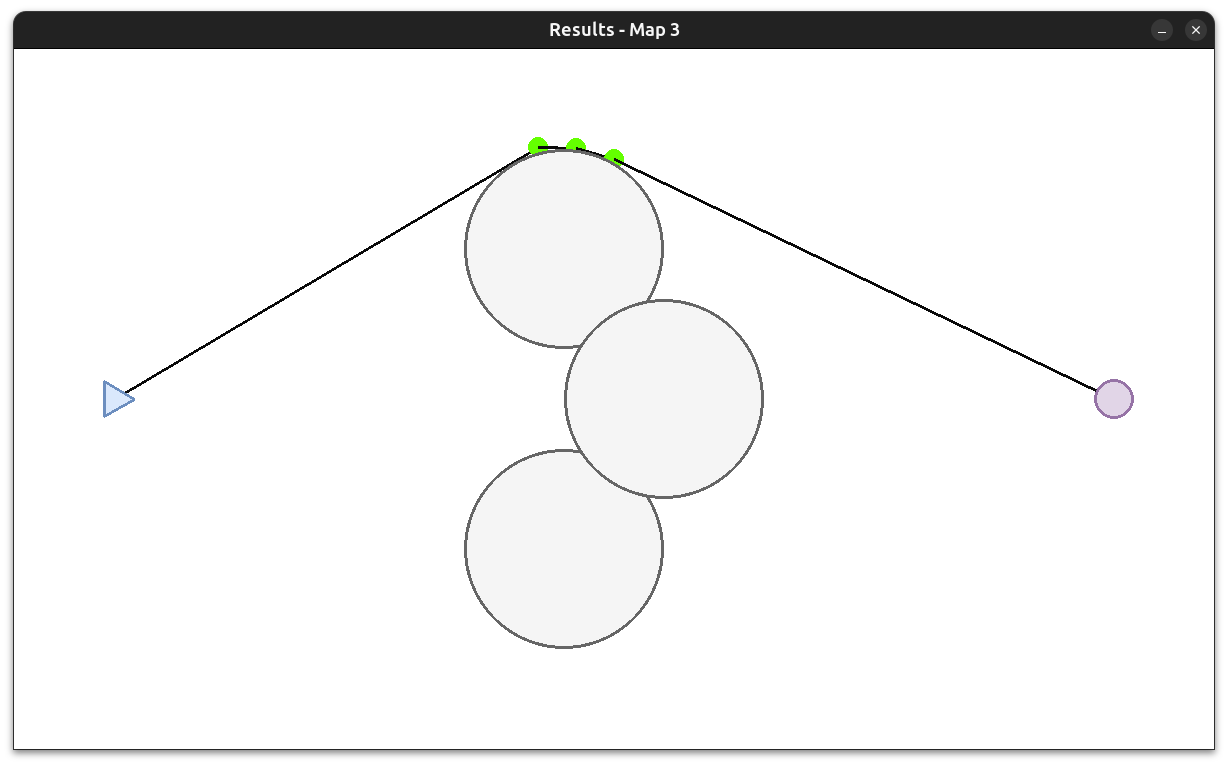
\includegraphics[width=\textwidth]{IMAGES/rmap3.png}
			\caption*{Résultat carte n°3}
			\label{fig:rmap3}
		\end{subfigure}
		\hfill
		\begin{subfigure}[b]{0.24\textwidth}
			\centering
			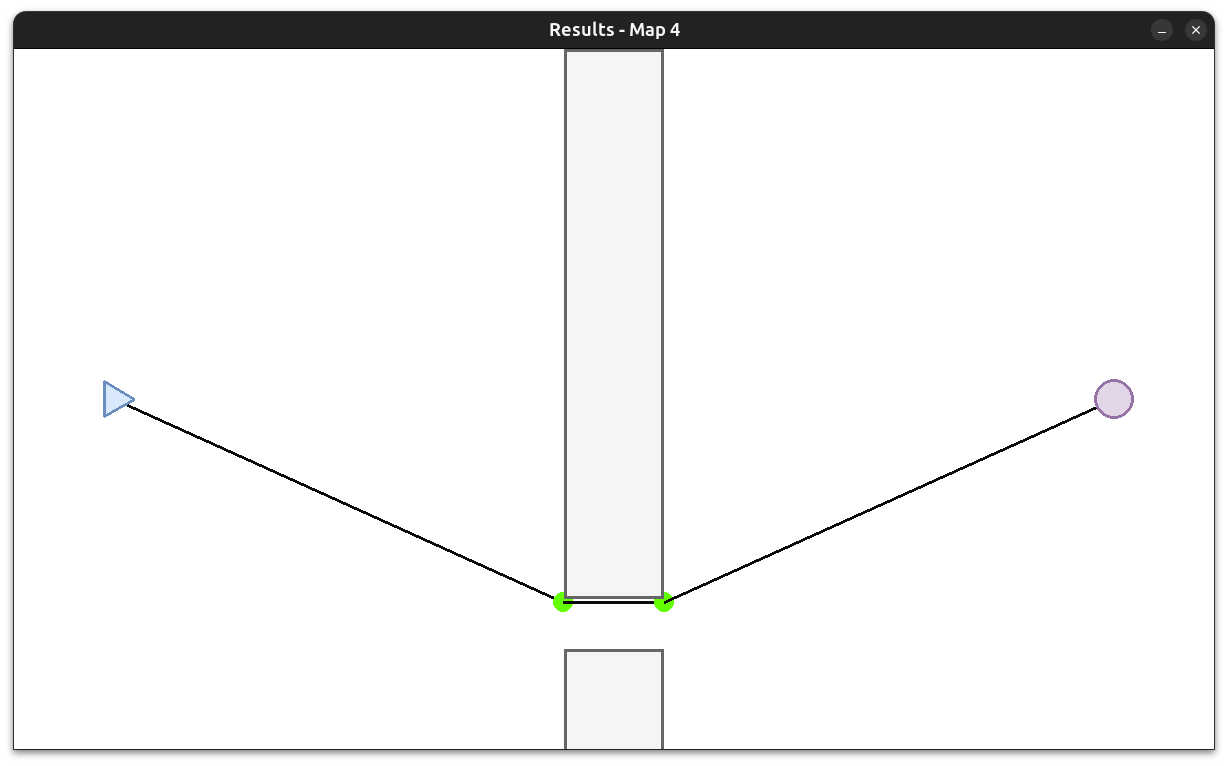
\includegraphics[width=\textwidth]{IMAGES/rmap4.png}
			\caption*{Résultat carte n°4}
			\label{fig:rmap4}
		\end{subfigure}
		\vfill
		\begin{subfigure}[b]{0.24\textwidth}
			\centering
			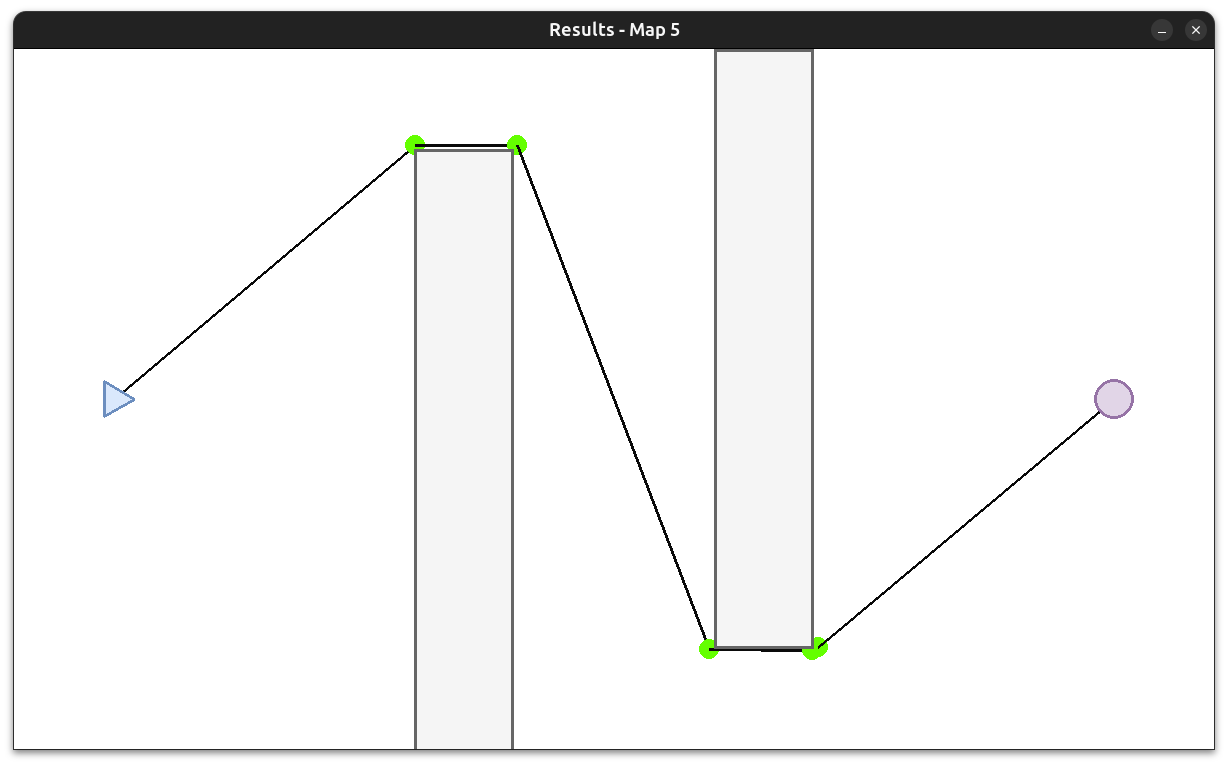
\includegraphics[width=\textwidth]{IMAGES/rmap5.png}
			\caption*{Résultat carte n°5}
			\label{fig:rmap5}
		\end{subfigure}
		\hfill
		\begin{subfigure}[b]{0.24\textwidth}
			\centering
			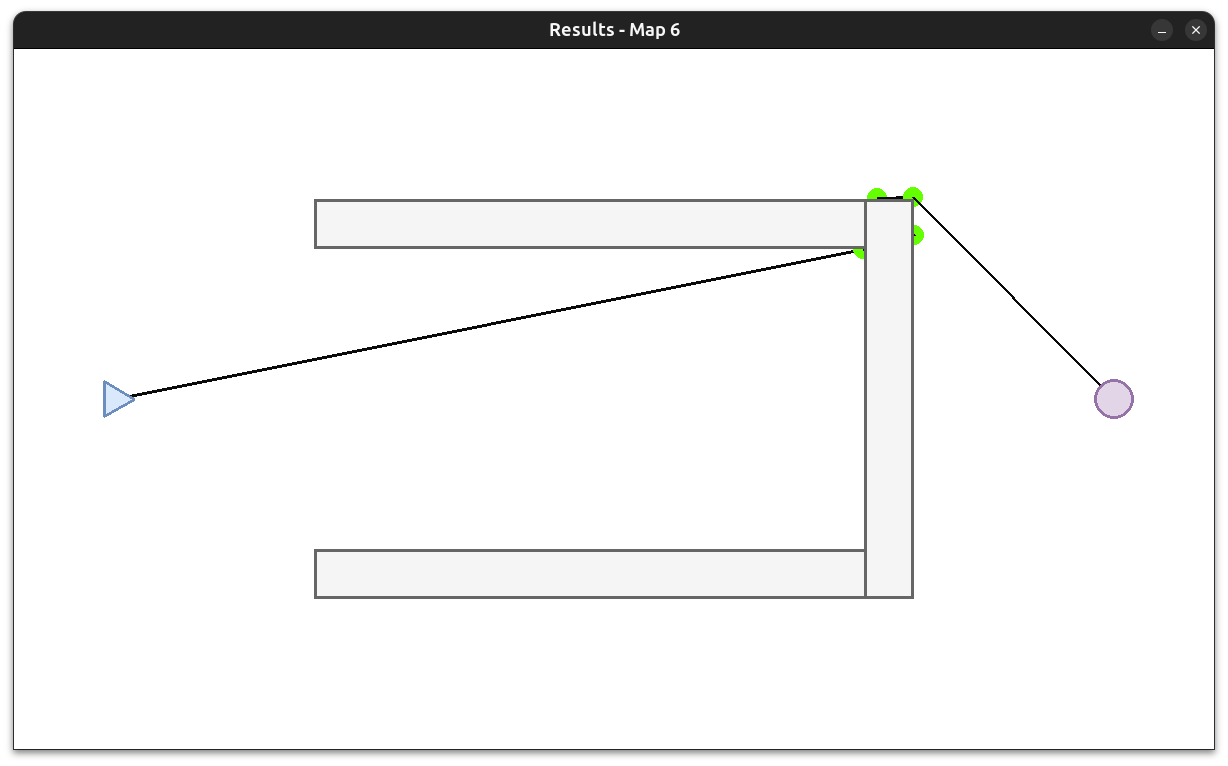
\includegraphics[width=\textwidth]{IMAGES/rmap6.png}
			\caption*{Résultat carte n°6}
			\label{fig:rmap6}
		\end{subfigure}
		\hfill
		\begin{subfigure}[b]{0.24\textwidth}
			\centering
			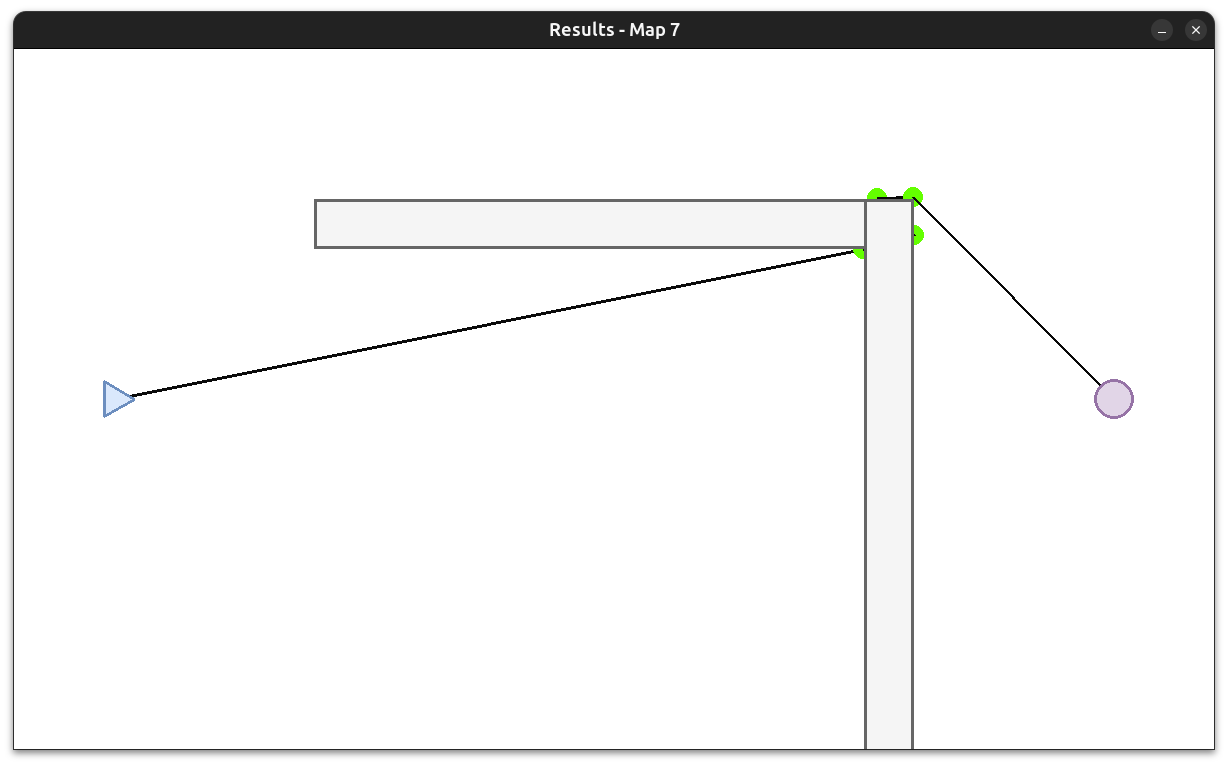
\includegraphics[width=\textwidth]{IMAGES/rmap7.png}
			\caption*{Résultat carte n°7}
			\label{fig:rmap7}
		\end{subfigure}
		\hfill
		\begin{subfigure}[b]{0.24\textwidth}
			\centering
			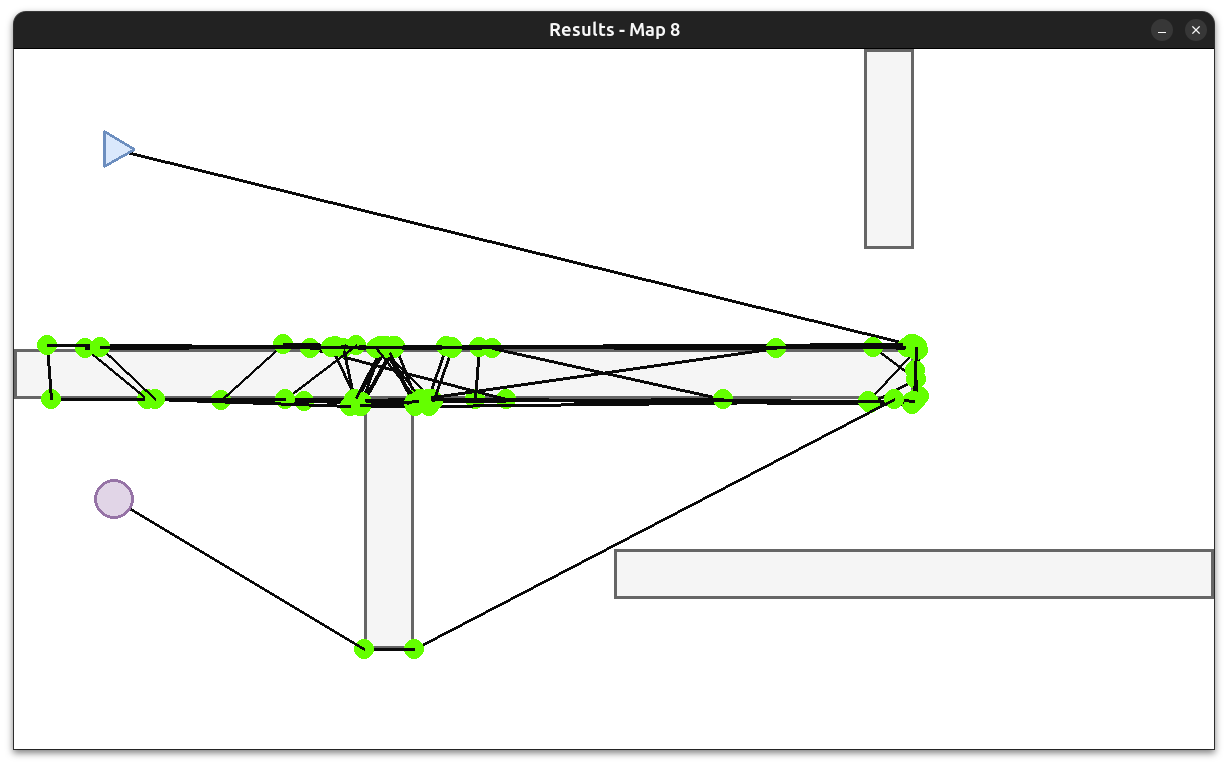
\includegraphics[width=\textwidth]{IMAGES/rmap8.png}
			\caption*{Résultat carte n°8}
			\label{fig:rmap8}
		\end{subfigure}
		\caption{Résultats sur les cartes de test}
		\label{fig:results_benchmark_maps}
	\end{figure}
\end{frame}

\begin{frame}{\textbf{Résultats et performance}}
    \begin{table}[H]
		\centering
		\begin{tabular}{c c c c c c}
			\hline
			Cartes & Théoriquement & Méthode & Rel. diff. ($\%$) & CA ($\pm 2$ mu) & Rel. Error ($\%$)\\
			\hline
			Carte 1 & 1081 & 1084 & 0.3 & 1086 & 0.5\\
			Carte 2 & 1121 & 1125 & 0.4 & 1122 & 0.1\\
			Carte 3 & 1122 & 1125 & 0.4 & 1122 & 0\\
			Carte 4 & 1084 & 1088 & 0.4 & 1086 & 0.2\\
			Carte 5 & 1521 & 1531 & 0.7 & 1522 & 0.1\\
			Carte 6 & 1166 & - & - & 1168 & 0.2\\
			Carte 7 & 1166 & - & - & 1168 & 0.2\\
			Carte 8 & 1776 & - & - & 1780 & 0.2\\
			\hline
		\end{tabular}
		\caption{Comparaisons des résultats}
		\label{tab:benchmark_results}
	\end{table}
\end{frame}

\begin{frame}{\textbf{Algorithme de Dijkstra}}
	\begin{itemize}
		\item Détection d'impasse :
		\vspace{0.2cm}
		\begin{itemize}
			\item Le robot reste dans un certain périmètre autour de sa position pendant un certain temps.
		\end{itemize}
		\vspace{0.2cm}
		\item En cas d'impasse :
		\vspace{0.2cm}
		\begin{itemize}
			\item Redéfinition du point étape :
			\vspace{0.2cm}
			\begin{itemize}
				\item Plus proche point appartenant aux cellules traversées de l'étape.
			\end{itemize}
			\vspace{0.2cm}
			\item Algorithme de Dijkstra :
			\vspace{0.2cm}
			\begin{itemize}
				\item Existence du chemin garanti.
			\end{itemize}
			\vspace{0.2cm}
			\item Simplification du chemin.
		\end{itemize}
	\end{itemize}

\end{frame}

\begin{frame}{\textbf{Analyses}}
	\begin{itemize}
		\item Portée délimitée d'application
		\vspace{0.2cm}
		\begin{itemize}
			\item Adaptée aux espaces ouverts et cavités moyennes.
			\item En cavités étroites, exécutions fréquentes de Dijkstra.
			\item Implémentation possible en 2D et 3D.
		\end{itemize}
		\vspace{0.2cm}
		\item Robustesse face aux pannes et à l'incertitude
		\vspace{0.2cm}
		\begin{itemize}
			\item Gestion des blocages et sortie de situations difficiles.
			\item Dijkstra assure un retour en arrière en cas de besoin.
		\end{itemize}
		\vspace{0.2cm}
		\item Complétude
		\vspace{0.2cm}
		\begin{itemize}
			\item Exploration de tout le domaine possible.
			\item Nécessité de tests approfondis.
			\item Complétude incertaine à ce stade.
		\end{itemize}
	\end{itemize}

\end{frame}


% Section 3 : Résultats
\section{Communication}

\begin{frame}{\textbf{Communication}}
	\textbf{Objectif}

	\vspace{0.5em}
	
	Coordonner l'exploration de zones inconnues par un essaim de robots, sans entité centrale pour gérer la coordination.
	
	\vspace{0.5em}

	\begin{itemize}
		\item Contraintes
		\begin{itemize}
			\item Environnement confiné
			\vspace{0.2cm}
			\item Liaisons souvent coupées
		\end{itemize}
		\vspace{0.2cm}
		\item Simplifications
		\begin{itemize}
			\item Communication possible si contact visuel
			\vspace{0.2cm}
			\item Pas de modélisation d'atténuation
			\vspace{0.2cm}
			\item Pas d'erreur de communication
		\end{itemize}
	\end{itemize}

\end{frame}

\begin{frame}{\textbf{Principe}}
	\begin{columns}
		\begin{column}{0.6\textwidth}
			\begin{itemize}
				\item Communication robot-à-robot :
				\begin{itemize}
					\item Communication par lumière.
				\end{itemize}
				\vspace{0.2cm}
				\item Sélection dynamique du robot maître :
				\begin{itemize}
					\item Le robot avec le plus petit ID devient le maître.
					% 	\item Si le groupe se divise, un maître est créé.
					% 	\item Si deux groupes se rencontre, les maîtres se synchronisent.
				\end{itemize}
				\vspace{0.2cm}
				\item Communication hiérarchique forte, le robot maître :
				\begin{itemize}
					\item donne des instructions aux robots avec un ID plus élevé.
					\item partage toutes les informations acquises par tout le groupe.
				\end{itemize}
			\end{itemize}
		\end{column}
		\begin{column}{0.4\textwidth}
			\begin{figure}
				\centering
				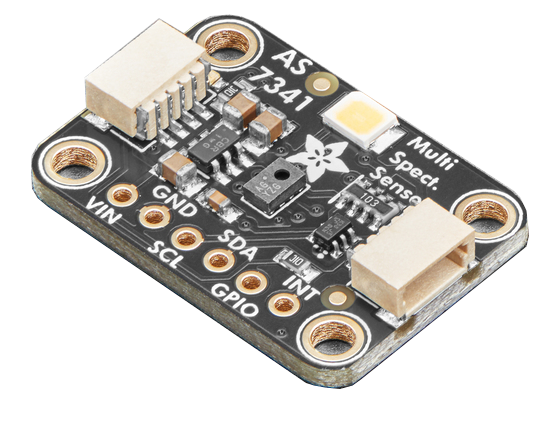
\includegraphics[width=0.4\textwidth]{IMAGES/color_sensor.png}
				\caption{Exemple de capteur de couleur, ref AS7341 - 10 cannaux}
				\label{fig:color_sensor}
			\end{figure}
		\end{column}
	\end{columns}
\end{frame}

\begin{frame}{\textbf{Principe}}
	\begin{columns}
		\begin{column}{0.5\textwidth}
			\begin{itemize}
				\item Choix des directions de groupe :
				\begin{itemize}
					\item Synchronisation de la carte connue.
					\vspace{0.2cm}
					\item Envoie des information du robot esclave vers le maître.
					\vspace{0.2cm}
					\item Calcul de la table de coût.
					\vspace{0.2cm}
					\item Envoie des directions par le maître en minimisant la combinaison des coût.
				\end{itemize}
			\end{itemize}
		\end{column}
		\begin{column}{0.5\textwidth}
			\begin{table}[H]
				\centering
				\begin{tabular}{c c c c c c}
					\hline
					& \textbf{R. 1} & \textbf{R. 2} & \textbf{R. 3} & \textbf{R. 4} & \textbf{R. 5}\\
					\hline
					\textbf{WP 1} & \textcolor{blue}{$\mathbf{23}$} & $87$ & $234$ & $56$ & $192$ \\
					\textbf{WP 2} & $245$ & $76$ & \textcolor{blue}{$\mathbf{11}$} & $68$ & $39$ \\
					\textbf{WP 3} & $90$ & \textcolor{blue}{$\mathbf{21}$} & $73$ & $\mathbf{50}$ & $164$ \\
					\textbf{WP 4} & $132$ & $58$ & $49$ & $77$ & \textcolor{blue}{$\mathbf{25}$} \\
					\textbf{WP 5} & $181$ & $\mathbf{13}$ & $66$ & \textcolor{blue}{$\mathbf{39}$} & $70$ \\ 
					\hline
				\end{tabular}
				\caption{Exemple de table de coût}
				\label{tab:example_5R5WP}
			\end{table}
			\begin{table}[H]
				\centering
				\begin{tabular}{c c c c c c}
					\hline
					& \textbf{R. 1} & \textbf{R. 2} & \textbf{R. 3} & \textbf{R. 4} & \textbf{R. 5}\\
					\hline
					\textbf{WP 1} & \textcolor{blue}{$\mathbf{61}$} & $125$ & $93$ & $47$ & \textcolor{blue}{$\mathbf{59}$} \\
					\textbf{WP 2} & $88$ & \textcolor{blue}{$\mathbf{12}$} & \textcolor{blue}{$\mathbf{53}$} & \textcolor{blue}{$\mathbf{29}$} & $174$ \\ 
					\hline
				\end{tabular}
				\caption{Autre exemple de table de coût}
				\label{tab:example_5R2WP}
			\end{table}
		\end{column}
	\end{columns}
\end{frame}


\begin{frame}{\textbf{Encodage}}
	\textbf{Structure d'un message type :}
	$$
	\underbrace{\smallsmile \smallsmile \smallsmile \smallsmile}_{\text{ID émetteur}}~~
	\underbrace{\smallsmile \smallsmile \smallsmile \smallsmile}_{\text{Nb de receveur}}~~
	\underbrace{\smallsmile \smallsmile \smallsmile \smallsmile \dots \smallsmile \smallsmile \smallsmile \smallsmile}_{4 \times \text{Nb de receveur}}~~
	\underbrace{\smallsmile \smallsmile \smallsmile \smallsmile \dots \smallsmile \smallsmile \smallsmile \smallsmile}_{\text{Message}}
	~~~ \cdots
	$$
	\vspace{0.3em}
	$$
	\cdots ~~~
	\underbrace{\smallsmile \smallsmile \smallsmile \smallsmile}_{\text{Indicateur de fin de message}}\;
	\underbrace{\smallsmile \smallsmile \smallsmile \smallsmile}_{\text{Verif. somme}}~~
	\underbrace{\smallsmile \smallsmile \smallsmile \smallsmile}_{\text{ID émetteur avec bit de parité}}
	$$

	\textbf{Resistance aux erreurs par methode ARQ}
\end{frame}


\begin{frame}{\textbf{Analyses}}
	\begin{itemize}
		\item{Portée délimitée d'application}
		\begin{itemize}
			\item Exploration robotique en essaim, scalabilité
			\item Intérieur ou extérieur
			\item Communication optique, propagation lumineuse
		\end{itemize}
		
		\vspace{0.2cm}
		\item{Robustesse face aux pannes et à l'incertitude}
		\begin{itemize}
			\item Detection d'erreurs (ARQ, vérification de somme, bit de parité)
			\item Réaffectation dynamique du rôle de maître
		\end{itemize}
		
		\vspace{0.2cm}
		\item{Vitesse}
		\begin{itemize}
			\item Encodage compact, bande passante réduite
			\item Cycle requête-réponse, réduire retransmissions
			\item Communication parallèle, traitement simultané
		\end{itemize}
	\end{itemize}
\end{frame}

% Section 4 : Discussions
\section{Simulateur et résultats}

\begin{frame}{\textbf{Simulateur}}
	\textbf{Objectif}

	\vspace{0.5em}

	Implementer et tester les algorithmes proposés pour les améliorer avant un déploiement sur robot
	
	\vspace{0.5em}

	\begin{itemize}
		\item Contraintes
		\begin{itemize}
			\item Simulateur en temps réel
			\vspace{0.2cm}
			\item Contrainte cinématique du robot prise en considération
		\end{itemize}
		\vspace{0.2cm}
		\item Simplifications
		\begin{itemize}
			\item Les robots opèrent dans les airs et se déplacent sur le sol
			\vspace{0.2cm}
			\item Le sol est approximé à un plan 2D
			\vspace{0.2cm}
			\item Aucune irrégularité de surface n'est prise en compte
		\end{itemize}
	\end{itemize}
\end{frame}

\begin{frame}{\textbf{Génération de la carte}}
	\begin{columns}[t]
		\begin{column}{0.33\textwidth}

			\vspace{1em}
			Génération des obstacles par automate cellulaire sur grille cartésienne
			\vspace{1em}
			
			\textbf{Règles :}

			\vspace{1em}

			Si 4 cellules sont actives dans le voisinage de Moore alors la cellule s'active sinon elle se désactive
		\end{column}

		\begin{column}{0.33\textwidth}
			\begin{figure}
				\centering
				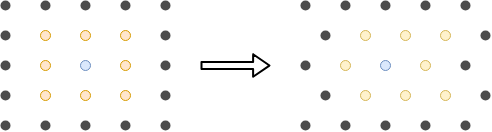
\includegraphics[width=0.9\textwidth]{IMAGES/grid_transform_map_generation.png}
				\caption{Transformation de la grille}
				\label{fig:map_generation_step3}
			\end{figure}
			\begin{figure}
				\centering
				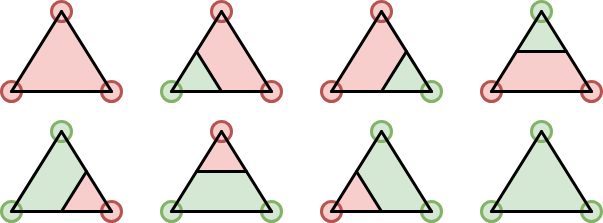
\includegraphics[width=0.9\textwidth]{IMAGES/marching_square_triangle.png}
				\caption{Méthode de Marching Square appliquée aux triangles}
				\label{fig:map_generation_step1}
			\end{figure}
		\end{column}
		\begin{column}{0.33\textwidth}
			\begin{figure}
				\centering
				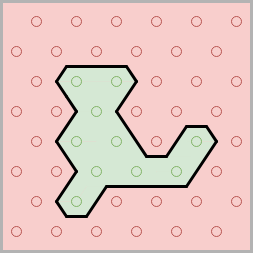
\includegraphics[width=0.8\textwidth]{IMAGES/map_generation_example.png}
				\caption{Exemple de carte générée}
				\label{fig:map_generation_step2}
			\end{figure}
		\end{column}
	\end{columns}
\end{frame}

\begin{frame}{\textbf{Exemple de cartes générées}}
    \begin{figure}[H]
		\centering
		\begin{subfigure}{0.32\textwidth}
			\centering
			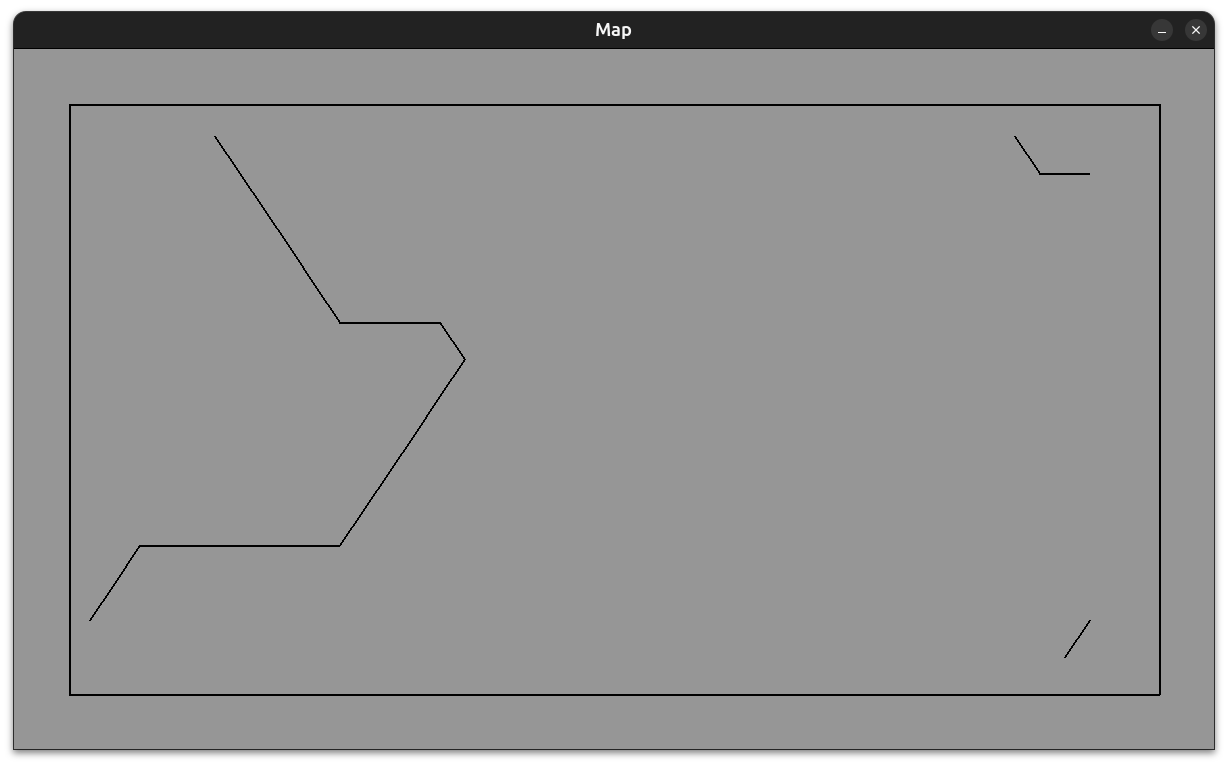
\includegraphics[width=\textwidth]{IMAGES/map_dx100.png}
			\caption{$\delta x = 100$ mu}
			\label{fig:real_map_100}
		\end{subfigure}
		\hfill
		\begin{subfigure}{0.32\textwidth}
			\centering
			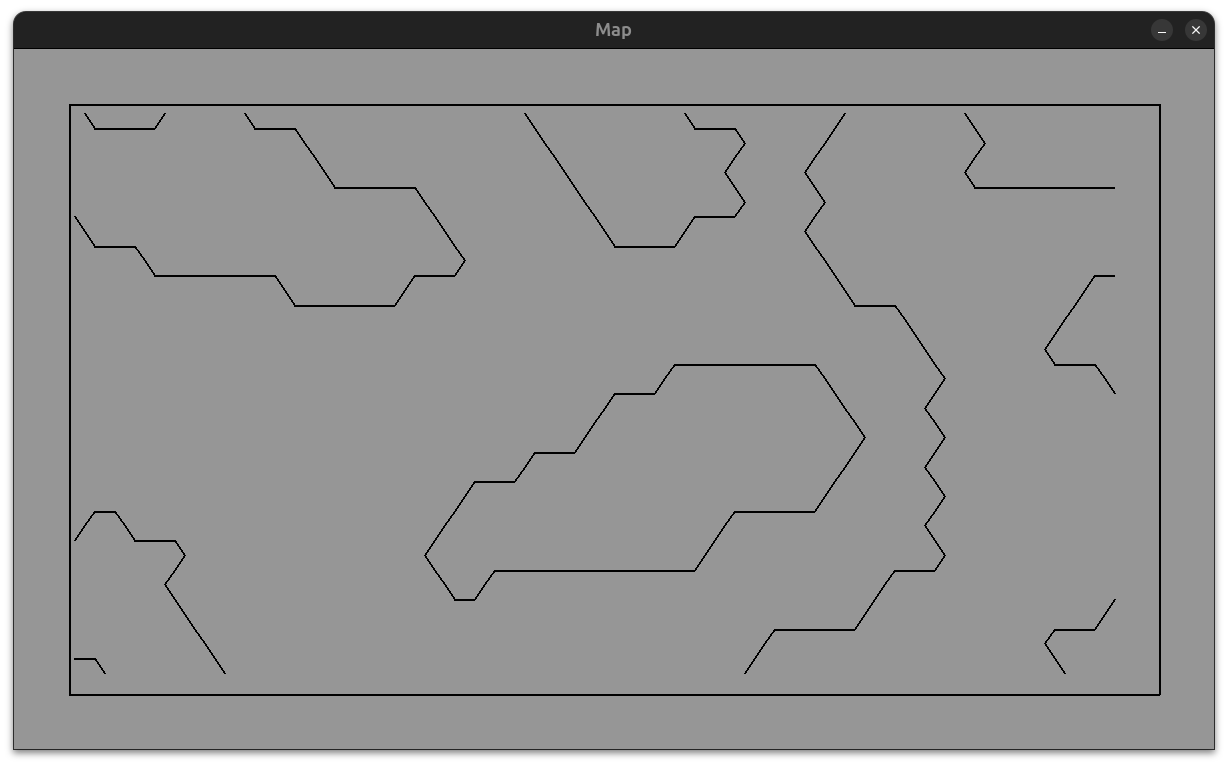
\includegraphics[width=\textwidth]{IMAGES/map_dx40.png}
			\caption{$\delta x = 40$ mu}
			\label{fig:real_map_40}
		\end{subfigure}
		\hfill
		\begin{subfigure}{0.32\textwidth}
			\centering
			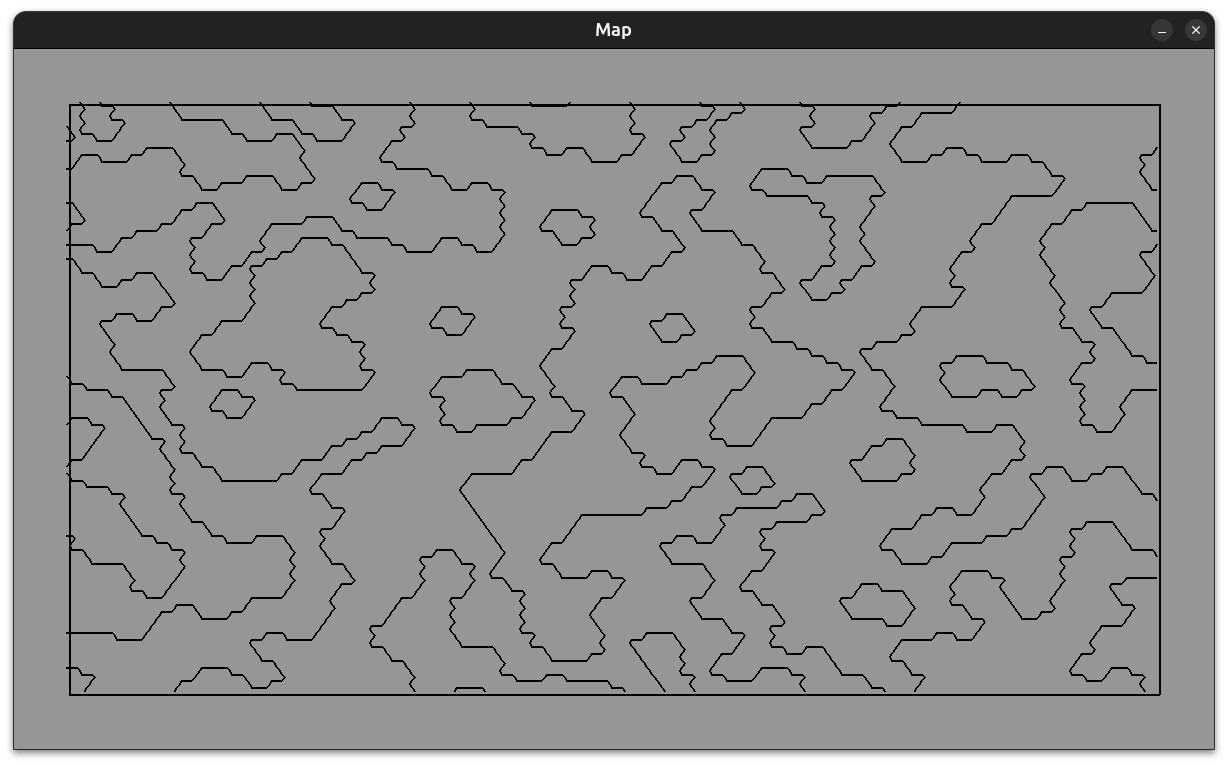
\includegraphics[width=\textwidth]{IMAGES/map_dx10.png}
			\caption{$\delta x = 10$ mu}
			\label{fig:real_map_10}
		\end{subfigure}
		\caption{Exemple de cartes générées}
		\label{fig:three_map_example}
	\end{figure}
\end{frame}

\begin{frame}{\textbf{Implémentation des capteurs}}
	\begin{columns}
		\begin{column}{0.5\textwidth}
			\begin{itemize}
				\item Centrale inertielle
				\vspace{0.2cm}
				\item LiDAR
				\begin{itemize}
					\item Émission
					\item Réflexion
					\item Réception
					\item Calcul du temps de vol $\rightarrow$ distance.
				\end{itemize}
				\vspace{0.2cm}
				\item Optimisations
				\begin{itemize}
					\item Segmentation de l'espace
					\item Algorithme de Bresenham modifié
				\end{itemize}
				\item Simulation des erreurs par loi normale
			\end{itemize}
		\end{column}
		\begin{column}{0.5\textwidth}
			\begin{figure}
				\centering
				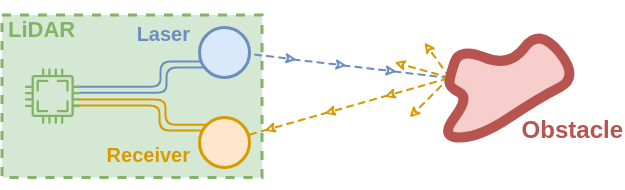
\includegraphics[width=0.6\textwidth]{IMAGES/lidar_operation_scheme.png}
				\caption{Fonctionnement d'un LiDAR}
				\label{fig:lidar_ope}
			\end{figure}
			\begin{figure}
				\centering
				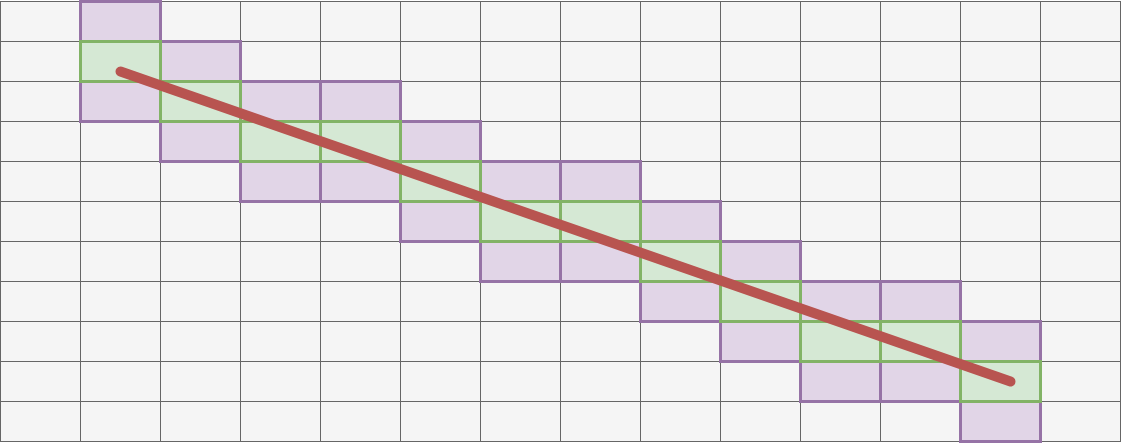
\includegraphics[width=0.6\textwidth]{IMAGES/draw_line.png}
				\caption{Algorithme de Bresenham modifié}
				\label{fig:bresenham_algorithm}
			\end{figure}
			
		\end{column}
	\end{columns}
\end{frame}


\begin{frame}{\textbf{Localisation et cartographie simultanées (SLAM)}}
	\begin{columns}[t]
		\begin{column}{0.5\textwidth}
			\begin{itemize}
				\item Création d'une carte de caractéristiques avec 4 états:
				\begin{itemize}
					\item Inconnue (Gris)
					\item Obstacle (Violet)
					\item Libre (Vert clair)
					\item Traversé (Vert)
				\end{itemize}				
			\end{itemize}
		\end{column}
		\begin{column}{0.5\textwidth}
			\begin{itemize}
			\item Calcul et correction de la position
				\begin{itemize}
					\item Centrale inertielle
					\item Triangulation par LiDAR
				\end{itemize}
			\end{itemize}
		\end{column}
	\end{columns}
	\begin{columns}[t]
		\begin{column}{0.5\textwidth}
			\begin{figure}
				\centering
				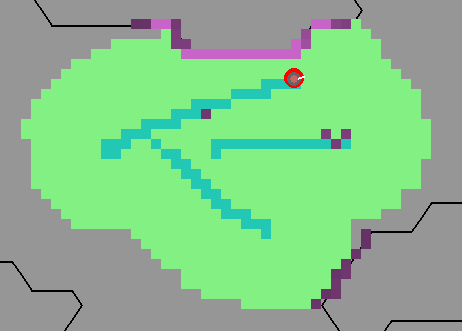
\includegraphics[width=0.5\textwidth]{IMAGES/lgm_t3_c.png}
				\caption{Carte des caractéristiques}
			\end{figure}
		\end{column}
		\begin{column}{0.5\textwidth}
			\begin{figure}
				\centering
				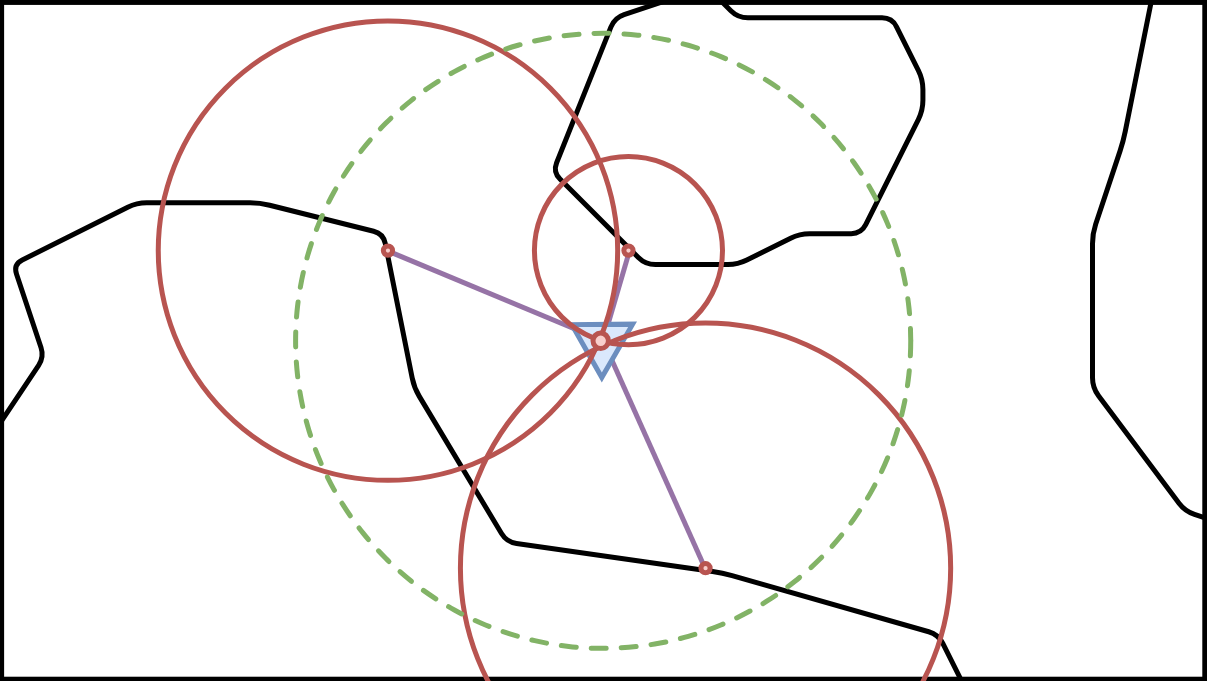
\includegraphics[width=0.6\textwidth]{IMAGES/lidar_correct_pos.png}
				\caption{Correction de la position par le LiDAR}
			\end{figure}
		\end{column}
	\end{columns}
		
\end{frame}

\begin{frame}{\textbf{Carte de caractéristiques dynamique}}
	\begin{columns}
		\begin{column}{0.7\textwidth}
			Environnement hautement dynamique
			\begin{itemize}
				\item Carte jumelle : carte d'occurrence
				\item Compte le nombre de rayons de LiDAR ayant touché les cellules de la carte de caractéristiques
				\begin{itemize}
					\item Si collision avec un mur : Ajouter 3
					\item Sinon : Soustraire 1
				\end{itemize}
			\end{itemize}
			\vspace{0.5em}
			
			Assure une carte des caractéristiques sécurisante tout en supprimant de celle-ci les objets dynamiques

			\begin{figure}[H]
				\centering
				\begin{subfigure}{0.32\textwidth}
					\centering
					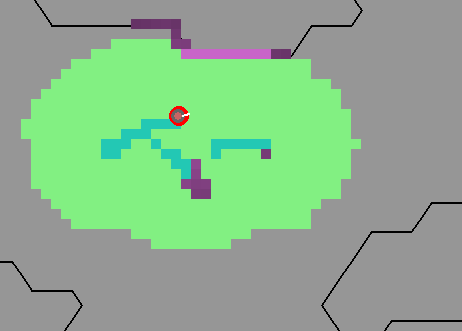
\includegraphics[width=0.6\textwidth]{IMAGES/lgm_t1_c.png}
				\end{subfigure}
				\hfill
				\begin{subfigure}{0.32\textwidth}
					\centering
					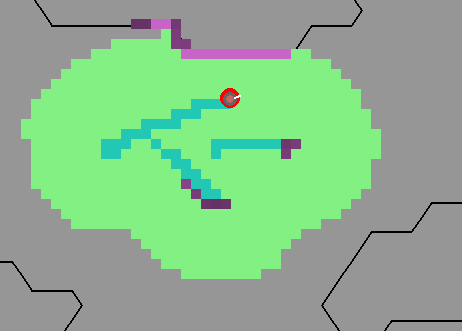
\includegraphics[width=0.6\textwidth]{IMAGES/lgm_t2_c.png}
				\end{subfigure}
				\hfill
				\begin{subfigure}{0.32\textwidth}
					\centering
					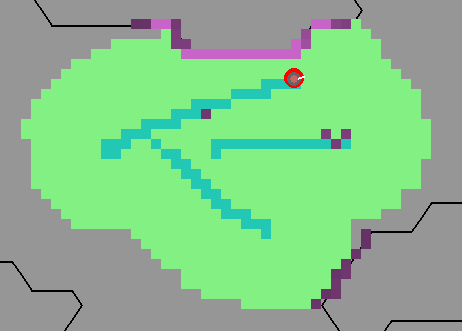
\includegraphics[width=0.6\textwidth]{IMAGES/lgm_t3_c.png}
				\end{subfigure}
			\end{figure}
			

			Amélioration possible : Filtre de Kalman
		\end{column}
		\begin{column}{0.3\textwidth}
			\begin{figure}
				\centering
				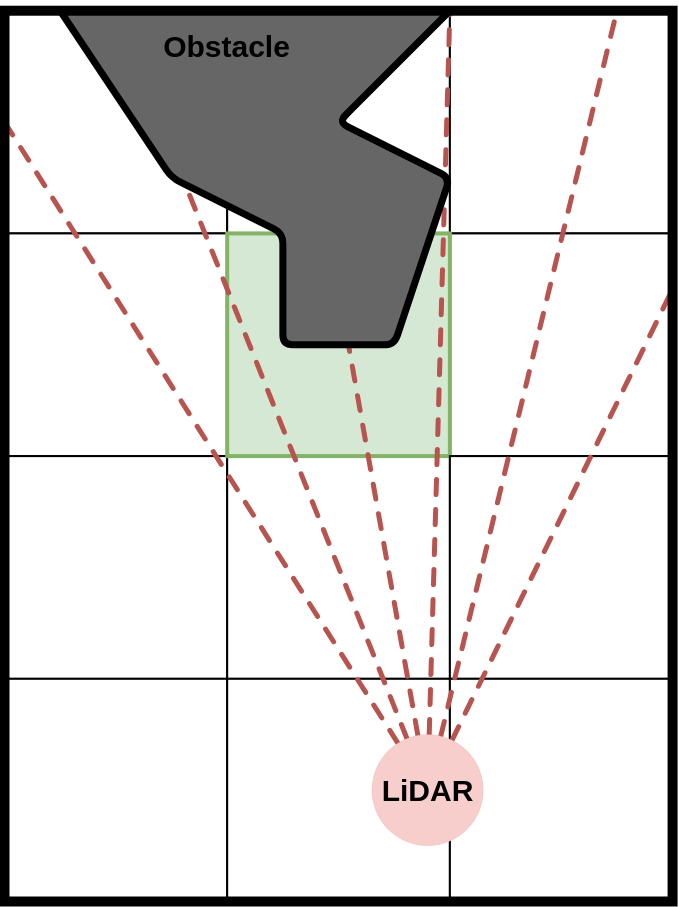
\includegraphics[width=0.6\textwidth]{IMAGES/lidar_occurance_map.png}
				\caption{Carte dynamique des caractéristiques}
			\end{figure}
		\end{column}
	\end{columns}

\end{frame}


\begin{frame}{\textbf{Résultats}}
	\begin{columns}
		\begin{column}{0.8\textwidth}
			\begin{table}[H]
				\centering
				\begin{tabular}{c c c c}
					\hline
					\textbf{Carte n°} & \textbf{Nb Robots} & \textbf{Temps exploration} & \textbf{Réduction} \\ 
					\hline
					30 & 1 & 2'20" & - \\
					30 & 2 & 1'3" & 55\% \\
					40 & 1 & 2'35" & - \\
					40 & 2 & 1'32" & 41\% \\
					55 & 1 & 2'7" & - \\
					55 & 2 & 54" & 57\% \\
					100 & 1 & 3'16" & - \\
					100 & 3 & 1'28" & 55\% \\
					100 & 5 & 1'12" & 63\% \\
				\end{tabular}
				\caption{Temps d'exploration pour différentes tailles de carte et nombre de robots}
				\label{tab:exploration_times_1}
			\end{table}
		\end{column}
		\begin{column}{0.2\textwidth}
			\begin{figure}[H]
				\centering
				\begin{subfigure}[b]{0.8\textwidth}
					\centering
					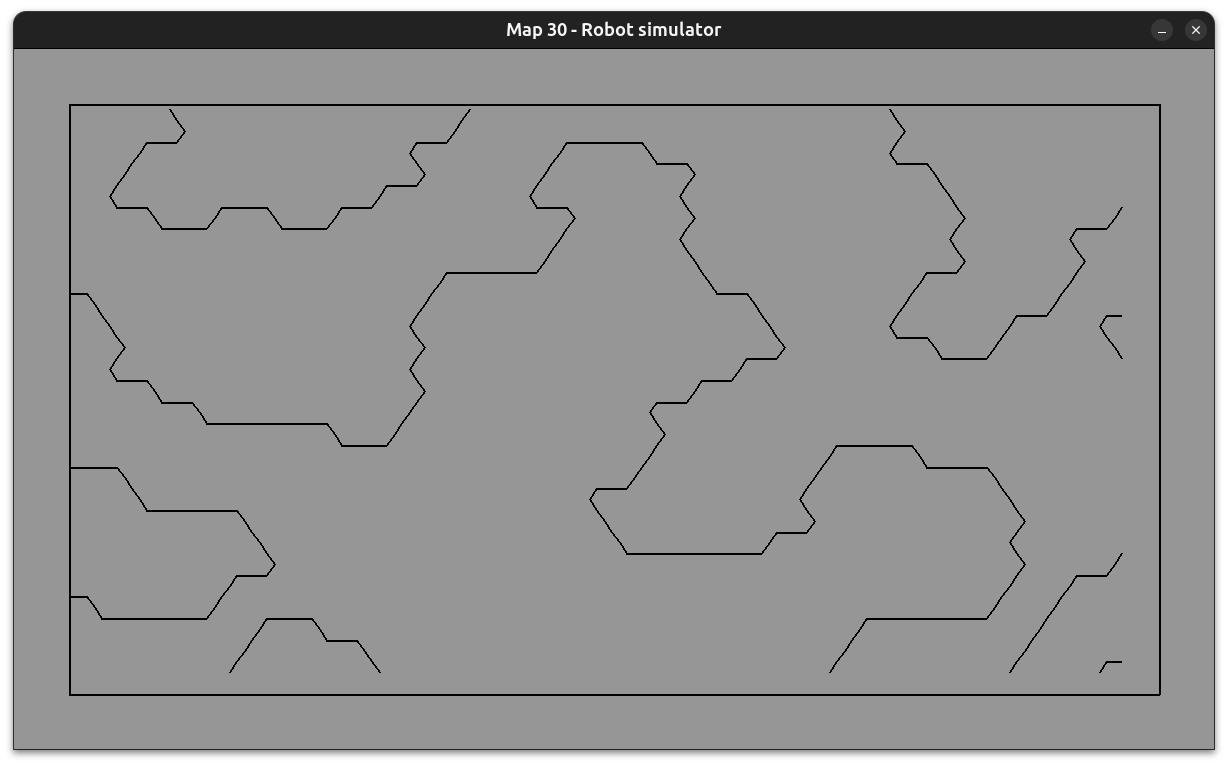
\includegraphics[width=\textwidth]{IMAGES/map30.png}
				\end{subfigure}
				\vfill
				\begin{subfigure}[b]{0.8\textwidth}
					\centering
					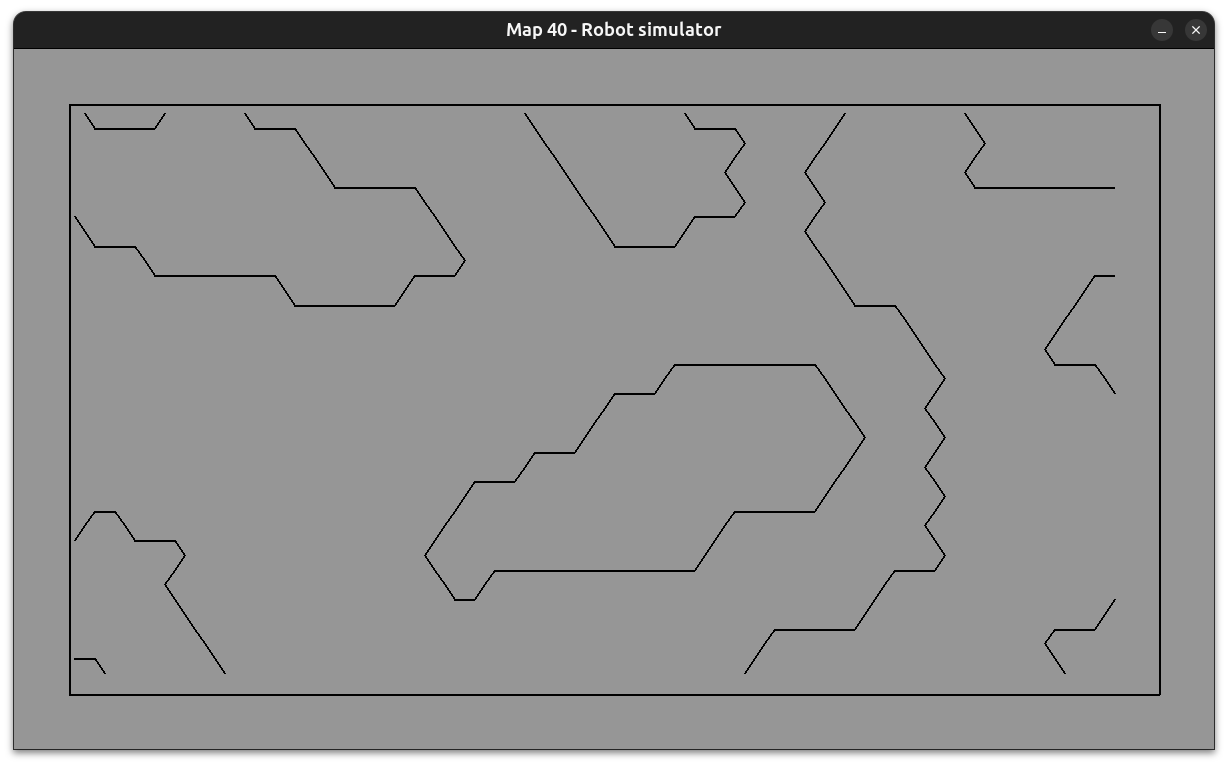
\includegraphics[width=\textwidth]{IMAGES/map40.png}
				\end{subfigure}
				\vfill
				\begin{subfigure}[b]{0.8\textwidth}
					\centering
					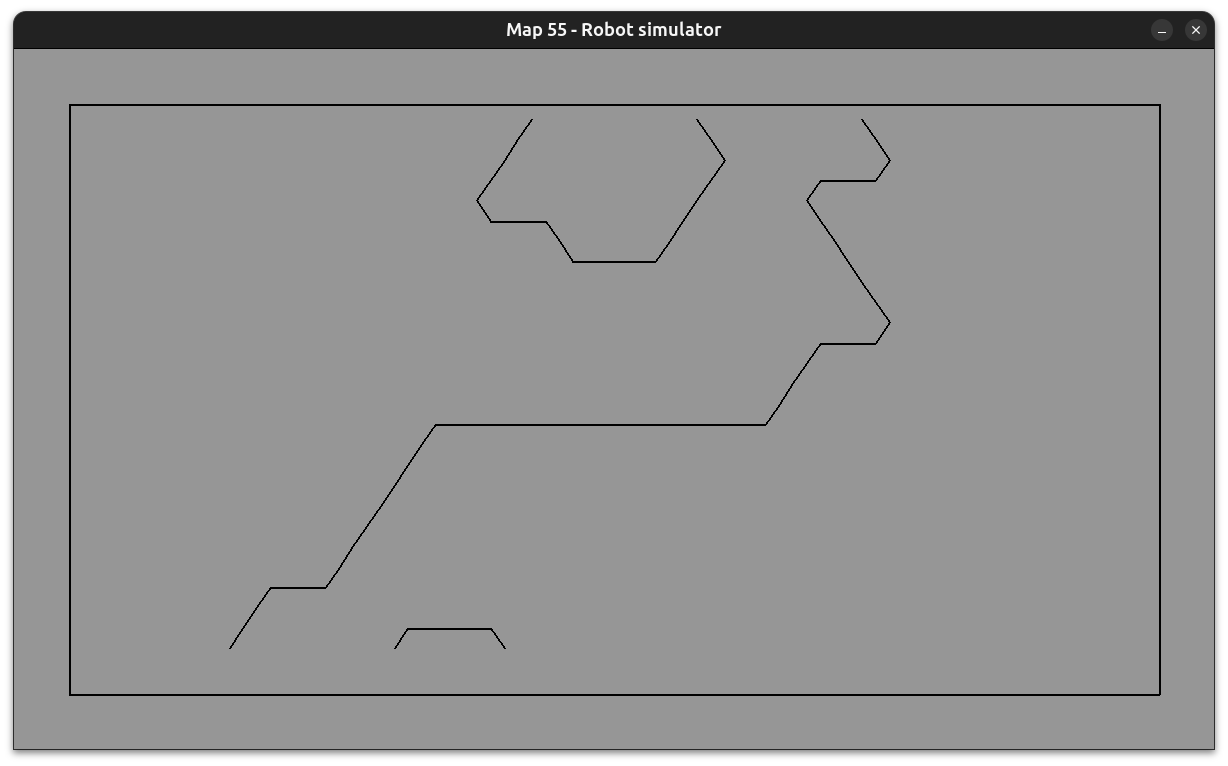
\includegraphics[width=\textwidth]{IMAGES/map55.png}
				\end{subfigure}
				\vfill
				\begin{subfigure}[b]{0.8\textwidth}
					\centering
					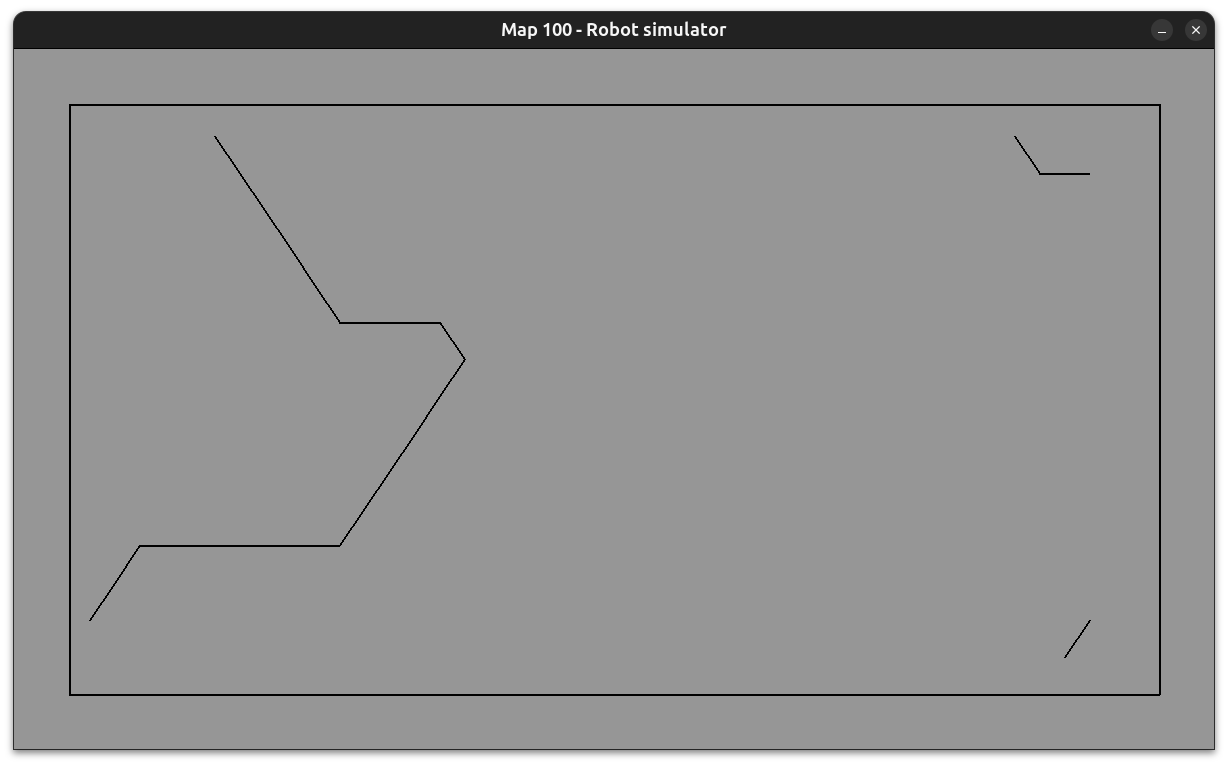
\includegraphics[width=\textwidth]{IMAGES/map100.png}
				\end{subfigure}
			\end{figure}
		\end{column}
	\end{columns}
\end{frame}

\begin{frame}{\textbf{Résultats}}
	\begin{columns}
		\begin{column}{0.33\textwidth}
			\begin{figure}[H]
				\centering
				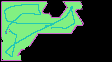
\includegraphics[width=0.9\textwidth]{IMAGES/map55_explored_2robot.png}
				\caption*{Carte n°55 - 2 robots}
			\end{figure}
		\end{column}
		\begin{column}{0.33\textwidth}
			\begin{figure}[H]
				\centering
				\begin{subfigure}{0.9\textwidth}
					\centering
					
\includegraphics[width=\textwidth]{IMAGES/map40_explored_1robot.png}
					\caption*{Carte n°40 - 1 robot}
				\end{subfigure}
				\vfill
				\begin{subfigure}{0.9\textwidth}
					\centering
					
\includegraphics[width=\textwidth]{IMAGES/map40_explored_2robot.png}
					\caption*{Carte n°40 - 2 robots}
				\end{subfigure}
			\end{figure}
		\end{column}
		\begin{column}{0.33\textwidth}
			\begin{figure}[H]
				\centering
				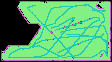
\includegraphics[width=0.9\textwidth]{IMAGES/map100_explored_5robot.png}
				\caption*{Carte n°100 - 5 robots}
			\end{figure}
		\end{column}
	\end{columns}
\end{frame}

% Section 5 : Conclusion
\section{Conclusion et perspectives}
\begin{frame}{\textbf{Conclusion}}
	\begin{itemize}
		\item Développement d'un simulateur :
		\begin{itemize}
			\item Environ 3500 lignes de code
			\item Une dizaine de fonctions utiles pour de futures implémentations
		\end{itemize}
		\vspace{0.2cm} 
		\item Validation des algorithmes d'exploration dans des environnements complexes
		\vspace{0.2cm} 
		\item Mise en place d'une communication simple mais robuste entre les robots
		\vspace{0.2cm} 
		\item Première étape vers des recherches approfondies en thèse
	\end{itemize}

\end{frame}


\begin{frame}{\textbf{Perspectives}}
	\begin{itemize}
		\item Amélioration de la performance du simulateur :
		\begin{itemize}
			\item Passage en C++
			\item Parallélisation
		\end{itemize}
		\vspace{0.2cm}
		\item Implémentation ROS
		\vspace{0.2cm}
		\item Implémentation du terrain
	\end{itemize}


\end{frame}

\begin{frame}{\textbf{Perspectives}}
    \begin{columns}[t]
        \begin{column}{0.55\textwidth}
            \textbf{Simplification du problème d'optimisation} \\
            \vspace{0.5em}
            \begin{itemize}
                \item Minimiser la consommation d'énergie lors du déplacement de A à B.
                \vspace{0.2cm}
                \item Consommation d'énergie : $\displaystyle E(T) = \int_{0}^{T} \| \omega(t) \| \, dt$
                \vspace{0.2cm}
                \item Où : $\| \omega(t) \| = \sqrt{\omega_L^{2}(t) + \omega_R^{2}(t)}$
                \vspace{0.2cm}
                \item Contraintes : \( X(0) = X_R \) et \( X(T) = X_{WP} \).
                \vspace{0.2cm}
                \item Problématique : Assurer \( X(T) = X_{WP} \).
            \end{itemize}
        \end{column}

        \begin{column}{0.45\textwidth}
			\begin{figure}[H]
				\centering
				\begin{subfigure}{0.45\textwidth}
					\centering
					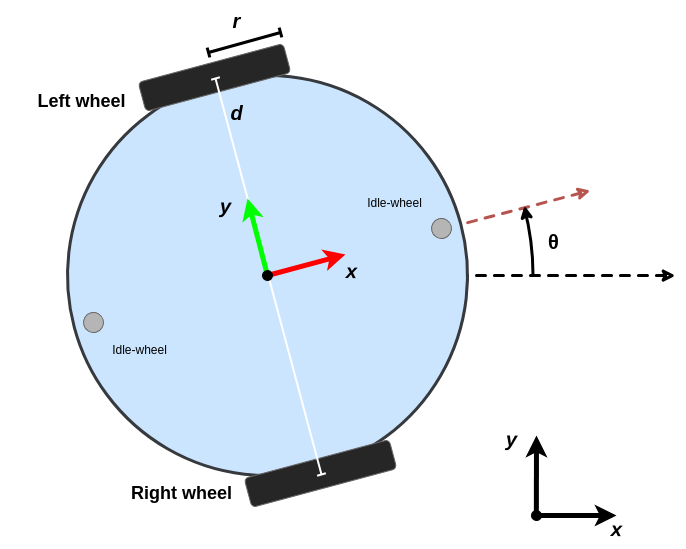
\includegraphics[width=\textwidth]{IMAGES/robot_model_2.png}
				\end{subfigure}
				\hfill
				\begin{subfigure}{0.45\textwidth}
					\centering
					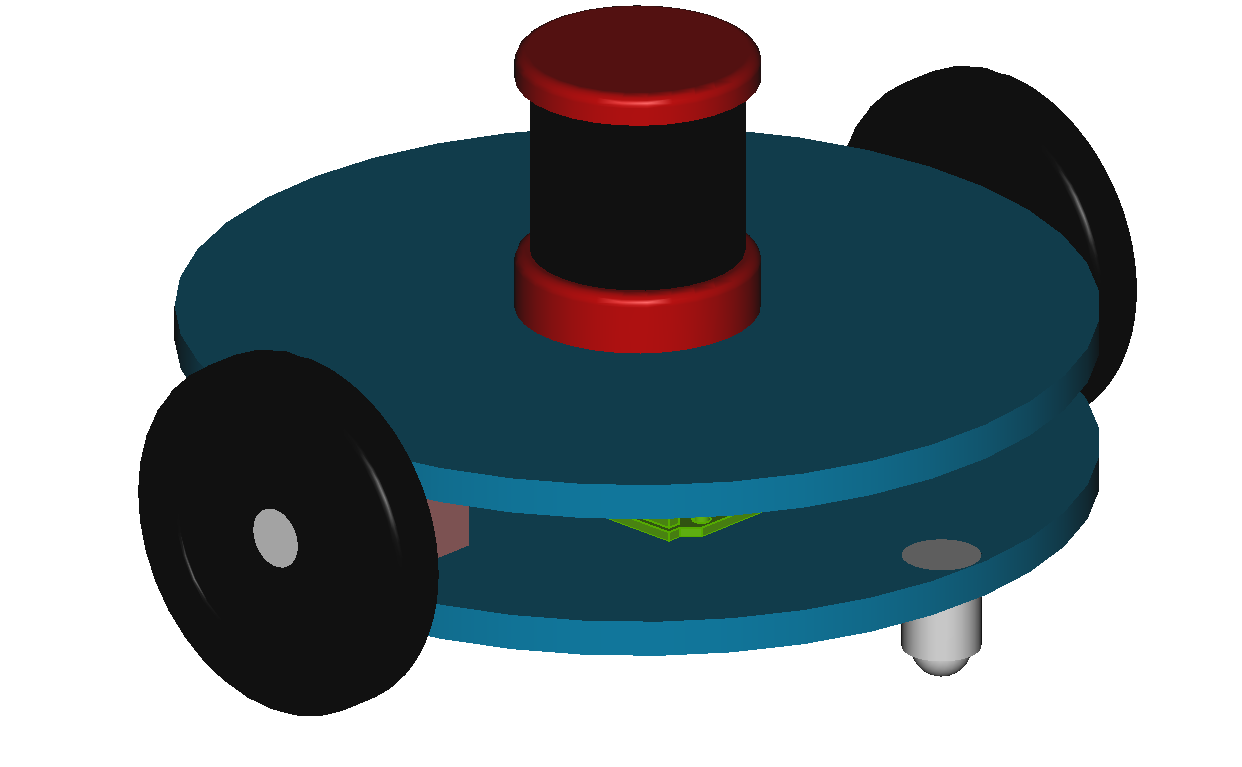
\includegraphics[width=\textwidth]{IMAGES/robot_3Dmodel.png}
				\end{subfigure}
				\caption{Modèle de robot utilisé}
			\end{figure}

            \begin{figure}[H]
                \centering
                \begin{subfigure}[b]{0.48\textwidth}
                    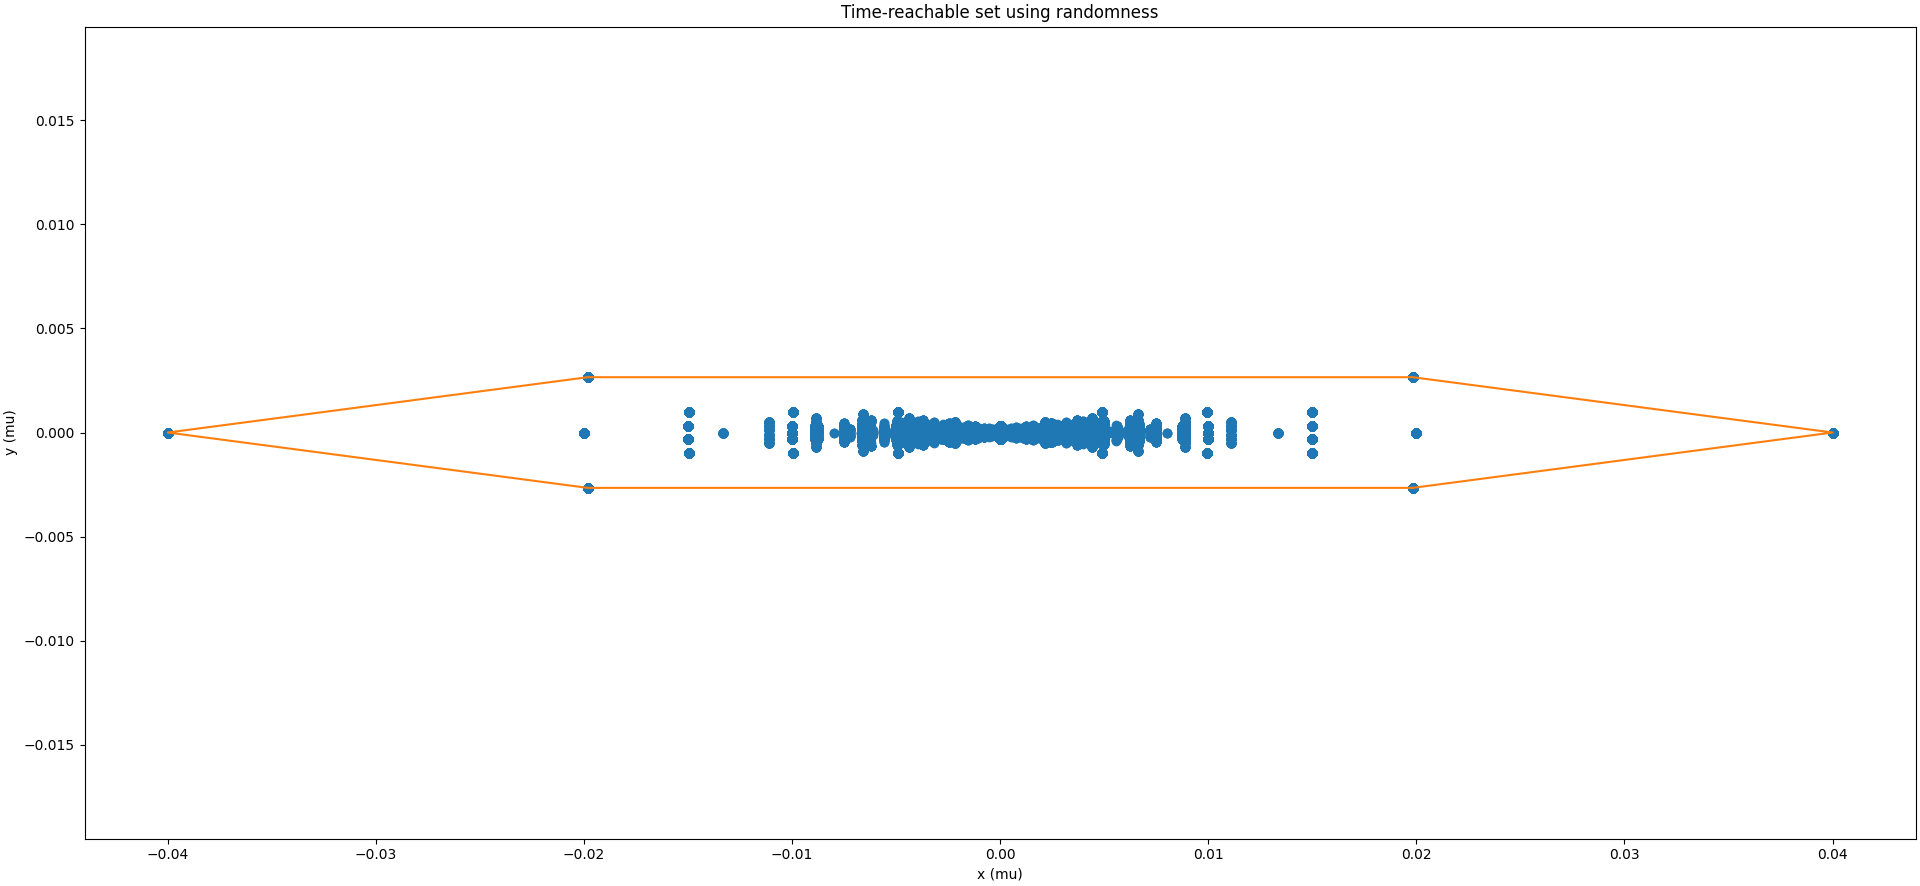
\includegraphics[width=\textwidth]{IMAGES/random.png}
                    \caption{Chemin stochastique}
                \end{subfigure}
                \hfill
                \begin{subfigure}[b]{0.48\textwidth}
                    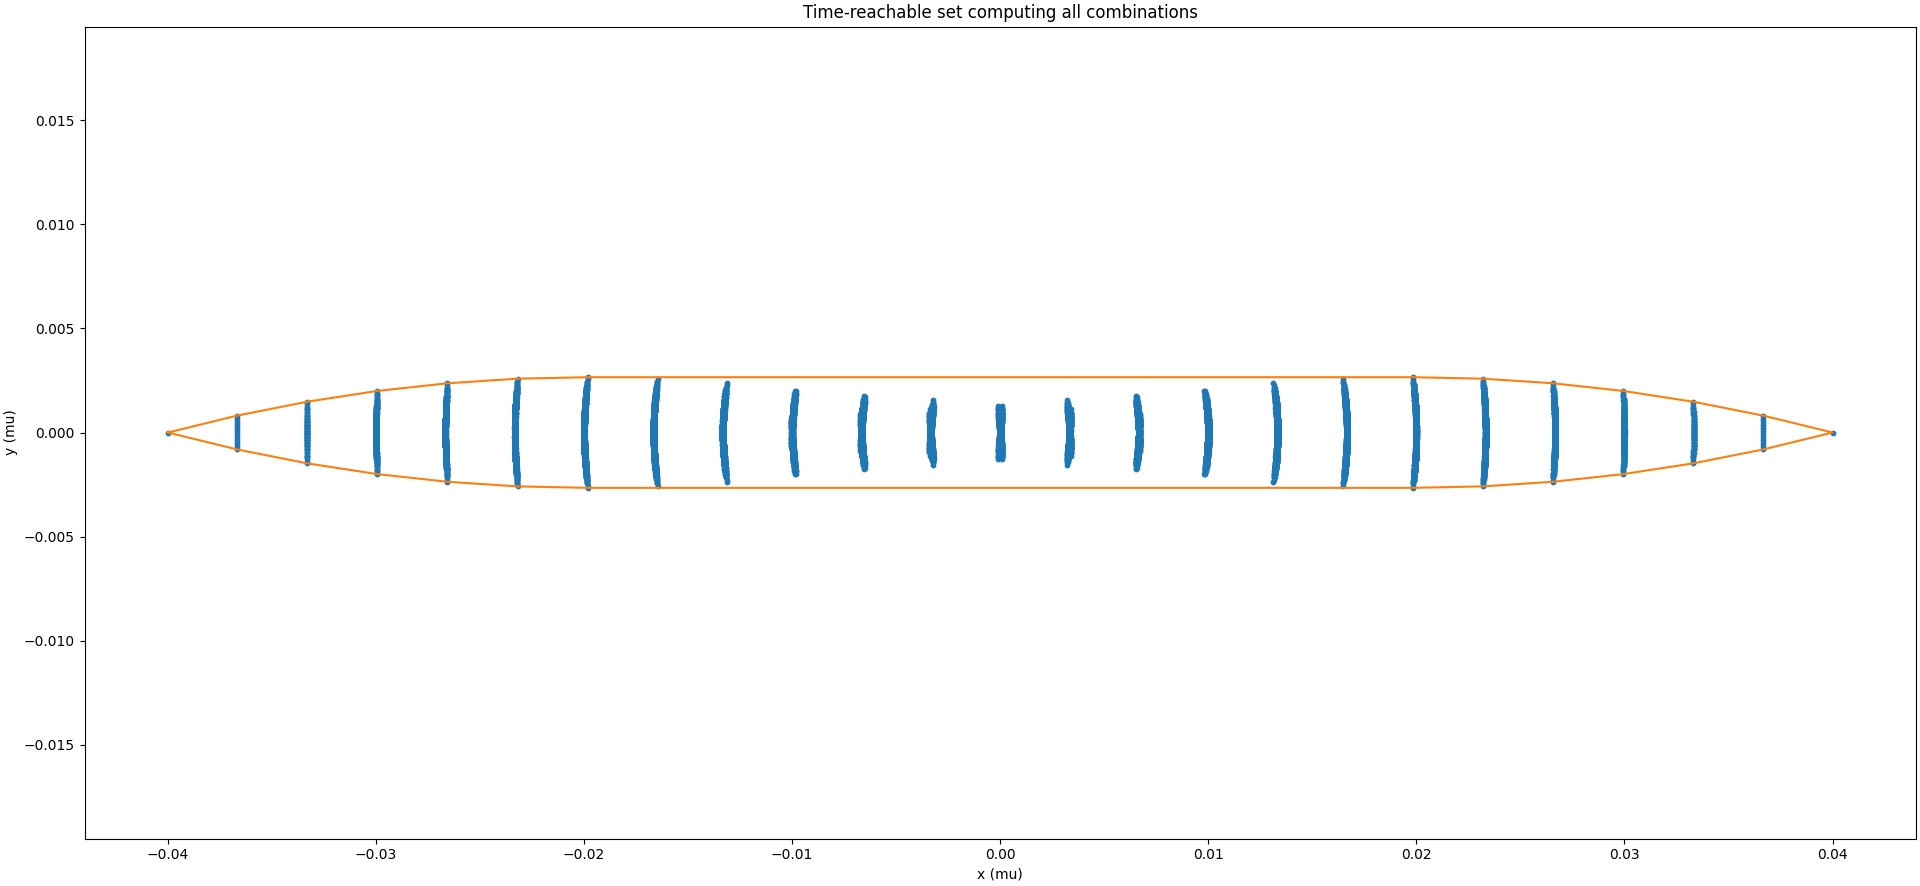
\includegraphics[width=\textwidth]{IMAGES/empiric.png}
                    \caption{Chemin empirique}
                \end{subfigure}
                \caption{Comparaison des approches d'optimisation des chemins stochastiques et empiriques}
            \end{figure}
        \end{column}
    \end{columns}
\end{frame}

\begin{frame}{\textbf{Références}}
	\scriptsize
	\begin{thebibliography}{9}

	\bibitem{tapia_2016}
	Calvo Tapia, Carlos, Villacorta-Atienza, José, Mironov, Vasily, Gallego, Victor, and Makarov, Valeri. (2016). WAVES in ISOTROPIC TOTALISTIC CELLULAR AUTOMATA: APPLICATION to REAL-TIME ROBOT NAVIGATION. \textit{Advances in Complex Systems}, 19, 1650012. DOI 10.1142/S0219525916500120.

	\end{thebibliography}

\end{frame}


\begin{frame}{\textbf{Table des types}}
    \begin{table}[H]
		\centering
		\begin{tabular}{c l l}
			\hline
			\textbf{Indicateur de type} & \textbf{Type} & \textbf{Taille des données}\\
			\hline
			\texttt{0000} & Fin de message & \texttt{4} bits\\
			\texttt{0001} & Entier & \texttt{8} bits\\
			\texttt{0010} & Entier & \texttt{32} bits\\
			\texttt{0011} & Flottant & \texttt{32} bits\\
			\texttt{0100} & Chaîne de caractères & \texttt{8} bits pour la longueur + \texttt{8} bits par caractère\\
			\texttt{0101} & Liste d'entiers 8 bits & \texttt{16} bits pour la longueur + \texttt{8} bits par entier\\
			\texttt{0110} & Liste de flottants & \texttt{16} bits pour la longueur + \texttt{32} bits par flottant\\
			\texttt{0111} & ID de type de message & \texttt{8} bits\\
			\texttt{1000} & Info robot & \texttt{168} bits\\
			\texttt{1010} & Message binaire & \texttt{16} bits pour la longueur + \texttt{1} bit par bit binaire\\
			\hline
		\end{tabular}
		\caption{Tableau des indicateurs de type}
	\end{table}
\end{frame}

\begin{frame}{\textbf{Table des identifiants de message}}
	\begin{table}[H]
		\centering
		\begin{tabular}{c l}
			\hline
			\textbf{Message ID} & \textbf{Description} \\
			\hline
			\texttt{00000000} & Demander de répéter le dernier message\\
			\texttt{00000001} & Dernier message reçu correctement\\[5pt]

			\texttt{00010000} & Demander l'ensemble des robots connectés\\
			\texttt{00010001} & Envoyer l'ensemble des robots connectés\\[5pt]

			\texttt{00100000} & Demander à tous où ils veulent aller\\
			\texttt{00100001} & Envoyer la position du prochain point de passage avec l'ID de la frontière\\
			\texttt{00100010} & Envoyer les informations du robot\\
			\texttt{00100011} & Envoyer la prochaine position à atteindre\\[5pt]

			\texttt{00110000} & Demander la synchronisation de la carte en direct\\
			\texttt{00110001} & Envoyer la carte en direct mise à jour\\[5pt]

			\texttt{01010101} & Transmettre un message d'un autre robot\\
			\hline
		\end{tabular}
		\caption{Table des identidiants de message}
	\end{table}
\end{frame}


\end{document}
